\begin{chapterpage}{Distributions of random variables}
  \chaptertitle[30]{Distributions of random \titlebreak{} variables}
  \label{ch_distributions}
  \chaptersection{normalDist}
\chaptersection{distributionofxbar}
  \chaptersection{geomDist}
  \chaptersection{binomialModel}
  \chaptersection{distributionphat}
\end{chapterpage}
\renewcommand{\chapterfolder}{ch_distributions}
\index{distribution!normal|(}
\index{normal distribution|}

\chapterintro{In this chapter, we discuss statistical distributions that frequently arise in the context of data analysis or statistical
  inference.  We start with the normal distribution in the first section,
  and we find that it is useful for approximating many of the other distributions introduced in the sections that follow. \vspace{6mm}

  \noindent%
  We also introduce the fundamental concept of a sampling distribution.  The sampling distribution of a sample proportion and of a sample mean underlie the inference procedures encountered in next chapters.}


%__________________________________________________
\section[Normal distribution]{Normal distribution}
\label{normalDist}

\sectionintro{
\noindent%
What proportion of adults have systolic blood pressure above 140?  What is the probability of getting more than 250 heads in 400 tosses of a fair coin?
If the average weight of a piece of carry-on luggage is 11 pounds, what is the probability that 200 random carry on pieces will weigh more than 2500 pounds?
If 55\% of a population supports a certain candidate, what is the probability that she will have less than 50\% support in a random sample of size 200? \vspace{3mm}

\noindent%
There is one distribution that can help us answer all of these questions.
Can you guess what it is?
That's right -- it's the normal distribution.

\subsection*{Learning objectives}
\begin{enumerate}
\setlength{\itemsep}{0mm}
\item Calculate and interpret a Z-score.

\item Understand that Z-scores are unitless (standard units) and are not affected by change of units.

\item Use the normal model to approximate a distribution where appropriate.

\item Find probabilities and percentiles using the normal approximation.

\item Find the value that corresponds to a given percentile when the distribution is approximately normal.  

\end{enumerate}
}


%%
\subsection{Normal distribution model}

Among all the distributions we see in practice, one is overwhelmingly the most common. The symmetric, unimodal, bell curve is ubiquitous throughout statistics. Indeed it is so common, that people often know it as the \term{normal curve} or \termsub{normal distribution}{distribution!normal}.\footnote{It is also introduced as the Gaussian distribution after Frederic Gauss, the first person to formalize its mathematical expression.} A normal curve is shown in Figure~\ref{simpleNormal}. 

\begin{figure}[h]
\centering
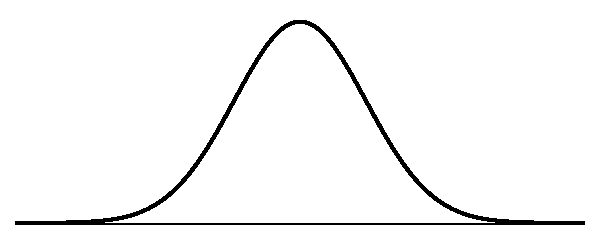
\includegraphics[width=0.6\textwidth]{ch_distributions/figures/simpleNormal/simpleNormal}
\caption{A normal curve.}
\label{simpleNormal}
\end{figure}

\D{\newpage}

The \term{normal distribution} always describes a symmetric, unimodal, bell-shaped curve. However, these curves can look different depending on the details of the model. Specifically, the normal distribution model can be adjusted using two parameters: mean and standard deviation. As you can probably guess, changing the mean shifts the bell curve to the left or right, while changing the standard deviation stretches or constricts the curve. Figure~\ref{twoSampleNormals} shows the normal distribution with mean $0$ and standard deviation $1$ in the left panel and the normal distributions with mean $19$ and standard deviation $4$ in the right panel. Figure~\ref{twoSampleNormalsStacked} shows these distributions on the same axis.


\begin{figure}[hht]
\centering
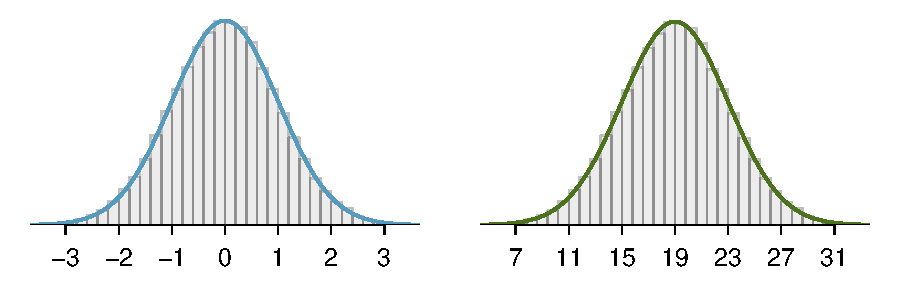
\includegraphics[width=0.95\textwidth]{ch_distributions/figures/twoSampleNormals/twoSampleNormals}
\caption{Both curves represent the normal distribution.  However, they differ in their center and spread. }
\label{twoSampleNormals}
\end{figure}

\begin{figure}[hht]
\centering
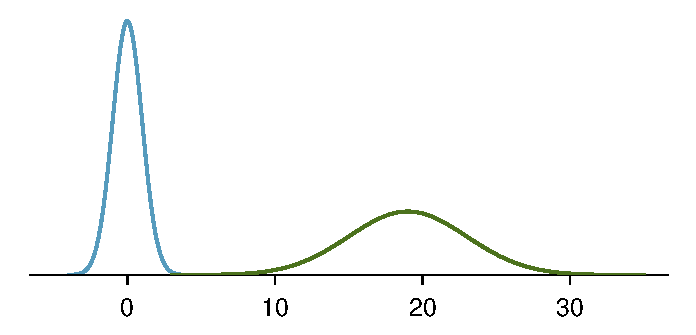
\includegraphics[width=0.67\textwidth]{ch_distributions/figures/twoSampleNormalsStacked/twoSampleNormalsStacked}
\caption{The normal distributions shown in Figure~\ref{twoSampleNormals} but plotted together and on the same scale.}
\label{twoSampleNormalsStacked}
\end{figure}

Because the mean and standard deviation describe a normal distribution exactly, they are called the distribution's \termsub{parameters}{parameter}.  The normal distribution with mean $\mu=0$ and standard deviation $\sigma = 1$ is called the \term{standard normal distribution}.%
\index{normal distribution!standard|textbf}.


\begin{onebox}{Normal distribution facts}
Many variables are nearly normal, but none are exactly normal. The normal distribution, while never perfect, provides very close approximations for a variety of scenarios. We will use it to model data as well as probability distributions.\vspace{0.7mm}\end{onebox}


\D{\newpage}

%%
\subsection{Standardizing with Z-scores}
\noindent%
We often want to put data onto a standardized scale,
which can make comparisons more reasonable.

\newcommand{\satmean}{1100}
\newcommand{\satsd}{200}
\newcommand{\actmean}{21}
\newcommand{\actsd}{6}
\newcommand{\annsatscore}{1300}
\newcommand{\annsatzscore}{1}
\newcommand{\tomsatscore}{24}
\newcommand{\tomsatzscore}{0.5}

\begin{examplewrap}
\begin{nexample}{Figure~\vref{satACTstats} shows the mean
    and standard deviation for total scores on the SAT and ACT.
    The distribution of SAT and ACT scores are both nearly normal.
    Suppose Ann scored \annsatscore{} on her SAT and Tom scored
    \tomsatscore{} on his ACT.
    Who performed better?}
  \label{actSAT}%
  We use the standard deviation as a guide.
  Ann is \annsatzscore{} standard deviation above average
  on the SAT: $\satmean{} + \satsd{} = \annsatscore{}$.
  Tom is \tomsatzscore{} standard deviations above the mean
  on the ACT:
  $\actmean{} + \tomsatzscore{} \times \actsd{} = \tomsatscore{}$.
  In Figure~\ref{satActNormals}, we can see that Ann tends
  to do better with respect to everyone else than Tom did,
  so her score was better.
\end{nexample}
\end{examplewrap}

\begin{figure}[h]
\centering
\begin{tabular}{l r r}
  \hline
  & SAT & ACT \\
  \hline
  Mean \hspace{0.3cm} & \satmean{} & \actmean{} \\
  SD & \satsd{} & \actsd{} \\
  \hline
\end{tabular}
\caption{Mean and standard deviation for the SAT and ACT.}
\label{satACTstats}
\end{figure}

\begin{figure}[h]
  \centering
  \Figure{0.61}{satActNormals}
  \caption{Ann's and Tom's scores shown with the distributions
      of SAT and ACT scores.}
  \label{satActNormals}
\end{figure}

Example~\ref{actSAT} used a standardization technique called
a Z-score, a method most commonly employed for nearly normal
observations but that may be used with any distribution.
Recall from Chapter 2 that the \term{Z-score} of an observation is defined
as the number of standard deviations it falls above or below
the mean.
If the observation is one standard deviation above the mean,
its Z-score is~1.
If it is 1.5 standard deviations \emph{below} the mean,
then its Z-score is -1.5.
If $x$ is an observation from a distribution with mean $\mu$ and standard deviation $\sigma$,
we define the Z-score mathematically as
\begin{align*}
Z = \frac{x - \mu}{\sigma}
\end{align*}
Using $\mu_{SAT} = \satmean{}$, $\sigma_{SAT} = \satsd{}$,
and $x_{_{\text{Ann}}} = \annsatscore{}$, we find Ann's Z-score:
\begin{align*}
Z_{_{\text{Ann}}}
  = \frac{x_{_{\text{Ann}}} - \mu_{_{\text{SAT}}}}
      {\sigma_{_{\text{SAT}}}}
  = \frac{\annsatscore{} - \satmean{}}{\satsd{}}
  = \annsatzscore{}
\end{align*}

\begin{exercisewrap}
\begin{nexercise}
Use Tom's ACT score, \tomsatscore{}, along with the ACT mean and
standard deviation to find his Z-score.\footnotemark{}
\end{nexercise}
\end{exercisewrap}
\footnotetext{$Z_{Tom}
  = \frac{x_{\text{Tom}} - \mu_{\text{ACT}}}
      {\sigma_{\text{ACT}}}
  = \frac{\tomsatscore{} - \actmean{}}{\actsd{}}
  = \tomsatzscore{}$}

%%
\subsection{Normal probability table}

\begin{examplewrap}
\begin{nexample}{Ann from Example~\ref{actSAT} earned a score of \annsatscore{} on her SAT with a corresponding $Z=1$. She would like to know what percentile she falls in among all SAT test-takers.}
Ann's \term{percentile} is the percentage of people who earned a lower SAT score than Ann. We shade the area representing those individuals in Figure~\ref{satBelow1300}. The total area under the normal curve is always equal to 1, and the proportion of people who scored below Ann on the SAT is equal to the \emph{area} shaded in Figure~\ref{satBelow1300}: 0.8413. In other words, Ann is in the $84^{th}$ percentile of SAT takers.
\end{nexample}
\end{examplewrap}

\begin{figure}[htb]
   \centering
   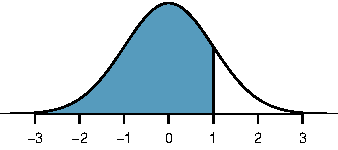
\includegraphics[width=0.45\textwidth]{ch_distributions/figures/satBelow1300/satBelow1300}
   \caption{The normal model for SAT scores, shading the area of those individuals who scored below Ann.}
   \label{satBelow1300}
\end{figure}

We can use the normal model to find percentiles. A \term{normal probability table}, which lists Z-scores and corresponding percentiles, can be used to identify a percentile based on the Z-score (and vice versa). Statistical software can also be used.

\D{\newpage}

A normal probability table is given in Appendix~\vref{normalProbabilityTable} and abbreviated in Figure~\ref{zTableShort}. We use this table to identify the percentile corresponding to any particular Z-score. For instance, the percentile of $Z=0.43$ is shown in row $0.4$ and column $0.03$ in Figure~\ref{zTableShort}: 0.6664, or the $66.64^{th}$ percentile. Generally, we round $Z$ to two decimals, identify the proper row in the normal probability table up through the first decimal, and then determine the column representing the second decimal value. The intersection of this row and column is the percentile of the observation.

\begin{figure}[h]
\centering
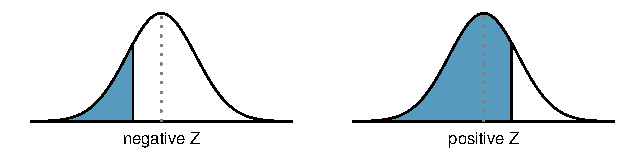
\includegraphics[width=0.7\textwidth]{ch_distributions/figures/normalTails/normalTails}
\caption{The area to the left of $Z$ represents the percentile of the observation.}
\label{normalTails}
\end{figure}

\begin{figure}[h]
\centering
\begin{tabular}{c | rrrrr | rrrrr |}
  \cline{2-11}
&&&& \multicolumn{4}{c}{Second decimal place of $Z$} &&& \\
  \cline{2-11}
$Z$ & 0.00 & 0.01 & 0.02 & 0.03 & \highlightO{0.04} & \highlightT{0.05
} & 0.06 & 0.07 & 0.08 & 0.09 \\
  \hline
  \hline
0.0 & \scriptsize{0.5000} & \scriptsize{0.5040} & \scriptsize{0.5080} & \scriptsize{0.5120} & \scriptsize{0.5160} & \scriptsize{0.5199} & \scriptsize{0.5239} & \scriptsize{0.5279} & \scriptsize{0.5319} & \scriptsize{0.5359} \\
  0.1 & \scriptsize{0.5398} & \scriptsize{0.5438} & \scriptsize{0.5478} & \scriptsize{0.5517} & \scriptsize{0.5557} & \scriptsize{0.5596} & \scriptsize{0.5636} & \scriptsize{0.5675} & \scriptsize{0.5714} & \scriptsize{0.5753} \\
  0.2 & \scriptsize{0.5793} & \scriptsize{0.5832} & \scriptsize{0.5871} & \scriptsize{0.5910} & \scriptsize{0.5948} & \scriptsize{0.5987} & \scriptsize{0.6026} & \scriptsize{0.6064} & \scriptsize{0.6103} & \scriptsize{0.6141} \\
%  May comment out 0.0-0.2 to make extra space. Then insert the following line:
%  $\vdots$ &   $\vdots$ &   $\vdots$ &   $\vdots$ &   $\vdots$ &   $\vdots$ &   $\vdots$ &   $\vdots$ &   $\vdots$ &   $\vdots$ &   $\vdots$ \\
  0.3 & \scriptsize{0.6179} & \scriptsize{0.6217} & \scriptsize{0.6255} & \scriptsize{0.6293} & \scriptsize{0.6331} & \scriptsize{0.6368} & \scriptsize{0.6406} & \scriptsize{0.6443} & \scriptsize{0.6480} & \scriptsize{0.6517} \\
\highlightT{0.4} & \scriptsize{0.6554} & \scriptsize{0.6591} & \scriptsize{0.6628} & \scriptsize{0.6664}& \scriptsize{0.6700} & \highlightT{\scriptsize{0.6736}} & \scriptsize{0.6772} & \scriptsize{0.6808} & \scriptsize{0.6844} & \scriptsize{0.6879} \\
  \hline
  0.5 & \scriptsize{0.6915} & \scriptsize{0.6950} & \scriptsize{0.6985} & \scriptsize{0.7019} & \scriptsize{0.7054} & \scriptsize{0.7088} & \scriptsize{0.7123} & \scriptsize{0.7157} & \scriptsize{0.7190} & \scriptsize{0.7224} \\
  0.6 & \scriptsize{0.7257} & \scriptsize{0.7291} & \scriptsize{0.7324} & \scriptsize{0.7357} & \scriptsize{0.7389} & \scriptsize{0.7422} & \scriptsize{0.7454} & \scriptsize{0.7486} & \scriptsize{0.7517} & \scriptsize{0.7549} \\
  0.7 & \scriptsize{0.7580} & \scriptsize{0.7611} & \scriptsize{0.7642} & \scriptsize{0.7673} & \scriptsize{0.7704} & \scriptsize{0.7734} & \scriptsize{0.7764} & \scriptsize{0.7794} & \scriptsize{0.7823} & \scriptsize{0.7852} \\
\highlightO{0.8} & \scriptsize{0.7881} & \scriptsize{0.7910} & \scriptsize{0.7939} & \scriptsize{0.7967} & \highlightO{\scriptsize{0.7995}} & \scriptsize{0.8023} & \scriptsize{0.8051} & \scriptsize{0.8078} & \scriptsize{0.8106} & \scriptsize{0.8133} \\
%  0.9 & \scriptsize{0.8159} & \scriptsize{0.8186} & \scriptsize{0.8212} & \scriptsize{0.8238} & \scriptsize{0.8264} & \scriptsize{0.8289} & \scriptsize{0.8315} & \scriptsize{0.8340} & \scriptsize{0.8365} & \scriptsize{0.8389} \\
%  \hline
%  \hline
%  1.0 & \scriptsize{0.8413} & \scriptsize{0.8438} & \scriptsize{0.8461} & \scriptsize{0.8485} & \scriptsize{0.8508} & \scriptsize{0.8531} & \scriptsize{0.8554} & \scriptsize{0.8577} & \scriptsize{0.8599} & \scriptsize{0.8621} \\
%  1.1 & \scriptsize{0.8643} & \scriptsize{0.8665} & \scriptsize{0.8686} & \scriptsize{0.8708} & \scriptsize{0.8729} & \scriptsize{0.8749} & \scriptsize{0.8770} & \scriptsize{0.8790} & \scriptsize{0.8810} & \scriptsize{0.8830} \\
  $\vdots$ &   $\vdots$ &   $\vdots$ &   $\vdots$ &   $\vdots$ &   $\vdots$ &   $\vdots$ &   $\vdots$ &   $\vdots$ &   $\vdots$ &   $\vdots$ \\
   \hline
\end{tabular}
\caption{A section of the normal probability table. The percentile for a normal random variable with $Z=0.45$ has been \highlightT{highlighted}, and the percentile closest to 0.8000 has also been \highlightO{highlighted}.}
\label{zTableShort}
\end{figure}

We can also find the Z-score associated with a percentile. For example, to identify Z for the $80^{th}$ percentile, we look for the value closest to 0.8000 in the middle portion of the table: 0.7995. We determine the Z-score for the $80^{th}$ percentile by combining the row and column Z values: 0.84.

\begin{exercisewrap}
\begin{nexercise}
Determine the proportion of SAT test takers who scored better than Ann on the SAT.\footnotemark
\end{nexercise}
\end{exercisewrap}
\footnotetext{If 84\% had lower scores than Ann, the proportion of people who had better scores must be 16\%. (Generally ties are ignored when the normal model, or any other continuous distribution, is used.)}


\D{\newpage}

%%
\subsection{Normal probability examples}

Cumulative SAT scores are approximated well by a normal model with mean \satmean{} and standard deviation \satsd{}.

\begin{examplewrap}
\begin{nexample}{What is the probability that a randomly selected SAT taker scores at least 1190 on the SAT?}\label{satAbove1190Exam}
The probability that a randomly selected SAT taker scores at least 1190 on the SAT is equivalent to the proportion of all SAT takers that score at least 1190 on the SAT. First, always draw and label a picture of the normal distribution. (Drawings need not be exact to be useful.) We are interested in the probability that a randomly selected score will be above 1190, so we shade this upper tail:
\begin{center}
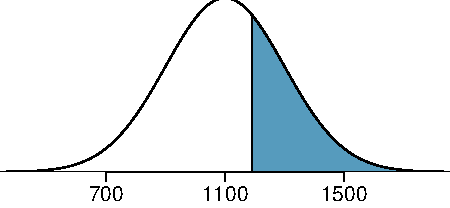
\includegraphics[height=0.9in]{ch_distributions/figures/satAbove1190/satAbove1190}
\end{center}
The picture shows the mean and the values at 2 standard deviations above and below the mean. The simplest way to find the shaded area under the curve makes use of the Z-score of the cutoff value. With $\mu=\satmean{}$, $\sigma=\satsd{}$, and the cutoff value $x=1190$, the Z-score is computed as
\begin{eqnarray*}
Z = \frac{x - \mu}{\sigma} = \frac{1190 - \satmean{}}{\satsd{}} = \frac{90}{200} = 0.45
\end{eqnarray*}
We look up the percentile of $Z=0.45$ in the normal probability table shown in Figure~\ref{zTableShort} or in Appendix~\vref{normalProbabilityTable}, which yields 0.6736. However, the percentile describes those who had a Z-score \emph{lower} than 0.45. To find the area \emph{above} $Z=0.45$, we compute one minus the area of the lower tail:
\begin{center}
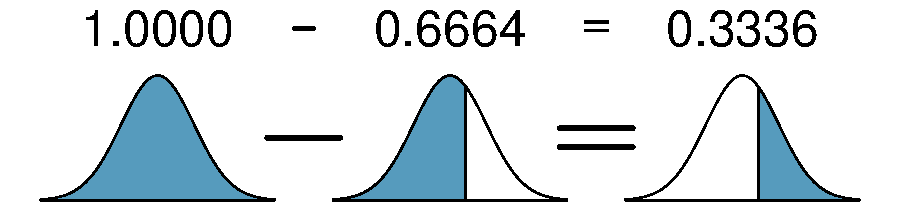
\includegraphics[height=0.8in]{ch_distributions/figures/subtractingArea/subtractingArea}
\end{center}
The probability that a randomly selected score is at least 1190 on the SAT is 0.3264.
\end{nexample}
\end{examplewrap}

\begin{onebox}{Always draw a picture first, and find the Z-score second}
For any normal probability situation, \emph{always always always} draw and label the normal curve and shade the area of interest first. The picture will provide an estimate of the probability. \vspace{3mm}

After drawing a figure to represent the situation, identify the Z-score for the observation of interest.\vspace{1mm}\end{onebox}

\begin{exercisewrap}
\begin{nexercise}
If the probability that a randomly selected score is at least 1190 is 0.3264, what is the probability that the score is less than 1190? Draw the normal curve representing this exercise, shading the lower region instead of the upper one.\footnotemark
\end{nexercise}
\end{exercisewrap}
\footnotetext{We found the probability in Example~\ref{satAbove1190Exam}: 0.6736. A picture for this exercise is represented by the shaded area below ``0.6736'' in Example~\ref{satAbove1190Exam}.}

\D{\newpage}

\begin{examplewrap}
\begin{nexample}{Edward earned a 1030 on his SAT. What is his percentile?} \label{edwardSatBelow1030}
First, a picture is needed. Edward's percentile is the proportion of people who do not get as high as a 1030. These are the scores to the left of 1030.
\begin{center}
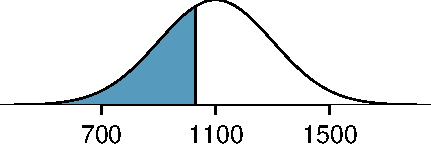
\includegraphics[height=22mm]{ch_distributions/figures/satBelow1030/satBelow1030}
\end{center}
Identifying the mean $\mu=1100$, the standard deviation $\sigma=200$, and the cutoff for the tail area $x=1030$ makes it easy to compute the Z-score:
\begin{eqnarray*}
Z = \frac{x - \mu}{\sigma} = \frac{1030 - 1100}{200} = -0.35
\end{eqnarray*}
Using the normal probability table, identify the row of $-0.3$ and column of $0.05$, which corresponds to the probability $0.3632$. Edward is at the $36^{th}$ percentile.
\end{nexample}
\end{examplewrap}

\begin{exercisewrap}
\begin{nexercise}
Use the results of Example~\ref{edwardSatBelow1030} to compute the proportion of SAT takers who did better than Edward. Also draw a new picture.\footnotemark
\end{nexercise}
\end{exercisewrap}
\footnotetext{If Edward did better than 36\% of SAT takers, then about 64\% must have done better than him. \\
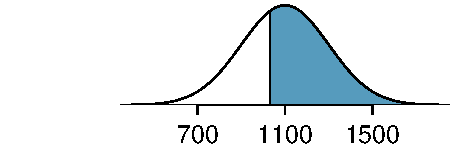
\includegraphics[width=0.35\textwidth]{ch_distributions/figures/satBelow1030/satAbove1030}}


\begin{onebox}{Areas to the right}
The normal probability table in most books gives the area to the left. If you would like the area to the right, first find the area to the left and then subtract this amount from~one.\end{onebox}

The last several problems have focused on finding the probability or percentile for a particular observation. It is also possible to identify the value corresponding to a particular percentile.

\D{\newpage}

\begin{examplewrap}
\begin{nexample}{Carlos believes he can get into his preferred college if he scores at least in the 80th percentile on the SAT. What score should he aim for?}
Here, we are given a percentile rather than a Z-score, so we work backwards. As always, first draw the picture.
\begin{center}
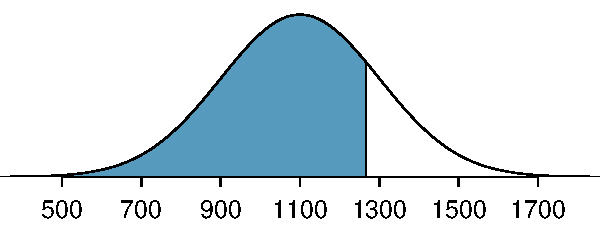
\includegraphics[height=22mm]{ch_distributions/figures/sat80thPercentile/sat80thPercentile}
\end{center}
We want to find the observation that corresponds to the 80th percentile. First, we find the Z-score associated with the 80th percentile using the normal probability table. Looking at Figure~\ref{zTableShort}., we look for the number closest to 0.80 \emph{inside} the table. The closest number we find is 0.7995 (highlighted). 0.7995 falls on row 0.8 and column 0.04, therefore it corresponds to a Z-score of 0.84. In any normal distribution, a value with a Z-score of 0.84 will be at the 80th percentile. Once we have the Z-score, we work backwards to find x.
\begin{align*}
Z &= \frac{x-\mu}{\sigma} \\
0.84 &= \frac{x-1100}{200} \\
0.84 \times 200+1100 &= x \\
x& = 1268
\end{align*}
The 80th percentile on the SAT corresponds to a score of 1268.
\end{nexample}
\end{examplewrap}

\begin{exercisewrap}
\begin{nexercise}Imani scored at the 72nd percentile on the SAT. What was her SAT score?\footnotemark\end{nexercise}
\end{exercisewrap}
\footnotetext{First, draw a picture! The closest percentile in the table to 0.72 is 0.7190, which corresponds to $Z = 0.58$. Next, set up the Z-score formula and solve for $x$: $0.58 = \frac{x-1100}{200} \rightarrow x = 1216$. Imani scored 1216.}


\begin{onebox}{If the data are not nearly normal, don't use a normal table}
{Before using the normal table, verify that the data or distribution is approximately normal. If it is not, the normal table will give incorrect results. Also, all answers based on normal approximations are approximations and are not exact.}
\end{onebox}



\D{\newpage}

%%
\subsection{Calculator: finding normal probabilities}
\label{normal}

\begin{onebox}{\videohref{ti84_normal_curve_area} TI-84: Finding area under the normal curve}
Use \calcbutton{2ND} \calcbutton{VARS}, \calctext{normalcdf} to find an area/proportion/probability between two Z-scores or to the left or right of a Z-score.\vspace{-1mm}
\begin{enumerate}
\setlength{\itemsep}{0mm}
\item Choose \calcbutton{2ND} \calcbutton{VARS} (i.e. \calctext{DISTR}).
\item Choose \calctext{2:normalcdf}.
\item Enter the \calctext{lower} (left) Z-score and the \calctext{upper} (right) Z-score.
\vspace{-1.5mm}
  \begin{itemize}
  \setlength{\itemsep}{0mm}
  \item If finding just a lower tail area, set \calctext{lower} to \calctext{-5}.
  \item If finding just an upper tail area, set \calctext{upper} to \calctext{5}.
\end{itemize}
\item Leave $\calctextmath{\mu}$ as \calctext{0} and $\calctextmath{\sigma}$ as \calctext{1}.
\item Down arrow, choose \calctext{Paste}, and hit \calcbutton{ENTER}.\vspace{-1.5mm}
\end{enumerate}
TI-83: Do steps 1-2, then enter the lower bound and upper bound separated by a comma, e.g. \calctext{normalcdf(2, 5)}, and hit \calcbutton{ENTER}.\end{onebox}

\begin{onebox}{\videohref{casio_normal_curve_area} Casio fx-9750GII: Finding area under the normal curve}
\begin{enumerate}
\setlength{\itemsep}{0mm}
\item Navigate to \calctext{STAT} (\calcbutton{MENU}, then hit \calcbutton{2}).
\item Select \calctext{DIST} (\calcbutton{F5}), then \calctext{NORM} (\calcbutton{F1}), and then \calctext{Ncd} (\calcbutton{F2}).
\item If needed, set \calctext{Data} to \calctext{Variable} (\calctext{Var} option, which is \calcbutton{F2}).
\item Enter the \calctext{Lower} Z-score and the \calctext{Upper} Z-score. Set $\calctextmath{\sigma}$ to \calctext{1} and $\calctextmath{\mu}$ to \calctext{0}.\vspace{-1.5mm}
  \begin{itemize}
  \setlength{\itemsep}{0mm}
  \item If finding just a lower tail area, set \calctext{Lower} to \calctext{-5}.
  \item For an upper tail area, set \calctext{Upper} to \calctext{5}.
  %\item If finding a middle area (e.g. $Z_{lower} = 0.5$ to $Z_{upper} = 1.5$), set the \calctext{lower} and \calctext{upper} values appropriately.
  \end{itemize}
\item Hit \calctext{EXE}, which will return the area probability (\calctext{p}) along with the Z-scores for the lower and upper bounds.
\end{enumerate}
\end{onebox}

\begin{examplewrap}
\begin{nexample}{Use a calculator to determine what percentile corresponds to a Z-score of 1.5.}
Always first sketch a graph:\footnotemark
\begin{center}
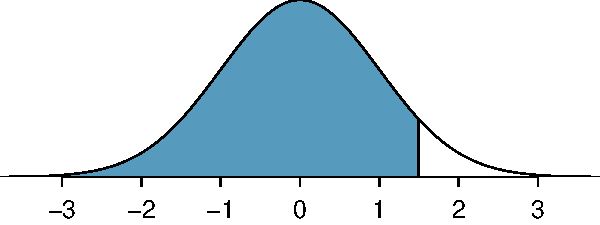
\includegraphics[width=0.5\textwidth]{ch_distributions/figures/zscoreleftof1point5/zscoreleftof1point5}\vspace{-2mm}
\end{center}
To find an area under the normal curve using a calculator, first identify a lower bound and an upper bound. Theoretically, we want all of the area to the left of 1.5, so the left endpoint should be -$\infty$. However, the area under the curve is nearly negligible when $Z$ is smaller than -4, so we will use -5 as the lower bound when not given a lower bound (any other negative number smaller than -5 will also work). Using a lower bound of -5 and an upper bound of 1.5, we get $P(Z < 1.5) = 0.933$.
\end{nexample}
\end{examplewrap}
\footnotetext{normalcdf gives the result without drawing the graph. To draw the graph, do 2nd VARS, DRAW, 1:ShadeNorm. However, beware of errors caused by other plots that might interfere with this plot.}

\begin{exercisewrap}
\begin{nexercise}
Find the area under the normal curve to right of $Z=2$.~\footnotemark
\end{nexercise}
\end{exercisewrap}
\footnotetext{Now we want to shade to the right. Therefore our lower bound will be 2 and the upper bound will be +5 (or a number bigger than 5) to get $P(Z > 2) = 0.023$.}

\begin{exercisewrap}
\begin{nexercise}Find the area under the normal curve between -1.5 and~1.5.~\footnotemark\end{nexercise}
\end{exercisewrap}
\footnotetext{Here we are given both the lower and the upper bound. Lower bound is -1.5 and upper bound is 1.5. The area under the normal curve between -1.5 and 1.5 = $P(-1.5 < Z < 1.5) = 0.866$.}


\begin{onebox}{\videohref{ti84_Z_score_for_a_percentile} TI-84: Find a Z-score that corresponds to a percentile}
\label{invNorm}
Use \calcbutton{2ND} \calcbutton{VARS}, \calctext{invNorm} to find the Z-score that corresponds to a given percentile.
\begin{enumerate}
\setlength{\itemsep}{0mm}
\item Choose \calcbutton{2ND} \calcbutton{VARS} (i.e. \calctext{DISTR}).
\item Choose \calctext{3:invNorm}.
\item Let \calctext{Area} be the percentile as a decimal (the area to the left of desired Z-score).
\item Leave $\calctextmath{\mu}$ as \calctext{0} and $\calctextmath{\sigma}$ as \calctext{1}.
\item Down arrow, choose \calctext{Paste}, and hit \calcbutton{ENTER}.\vspace{-1.5mm}
\end{enumerate}
TI-83: Do steps 1-2, then enter the percentile as a decimal, e.g.~\mbox{\calctext{invNorm(.40)},} then hit \calcbutton{ENTER}.\end{onebox}

\begin{onebox}{\videohref{casio_Z_score_for_a_percentile} Casio fx-9750GII: Find a Z-score that corresponds to a percentile}
\begin{enumerate}
\setlength{\itemsep}{0mm}
\setlength{\itemsep}{0mm}
\item Navigate to \calctext{STAT} (\calcbutton{MENU}, then hit \calcbutton{2}).
\item Select \calctext{DIST} (\calcbutton{F5}), then \calctext{NORM} (\calcbutton{F1}), and then \calctext{InvN} (\calcbutton{F3}).
\item If needed, set \calctext{Data} to \calctext{Variable} (\calctext{Var} option, which is \calcbutton{F2}).
\item Decide which tail area to use (\calctext{Tail}), the tail area (\calctext{Area}), and then enter the $\calctextmath{\sigma}$ and $\calctextmath{\mu}$ values.
\item Hit \calctext{EXE}.
\end{enumerate}
\end{onebox}

\begin{examplewrap}
\begin{nexample}{Use a calculator to find the Z-score that corresponds to the 40th percentile.}Letting Area be 0.40, a calculator gives -0.253. This means that $Z = -0.253$ corresponds to the 40th percentile, that~is, $P(Z < -0.253) = 0.40$.
\end{nexample}
\end{examplewrap}

\begin{exercisewrap}
\begin{nexercise}Find the Z-score such that 20 percent of the area is to the right of that Z-score.\footnotemark\end{nexercise}
\end{exercisewrap}	
\footnotetext{If 20\% of the area is the right, then 80\% of the area is to the left. Letting area be 0.80, we get $Z = 0.841$.}

\D{\newpage}

\begin{examplewrap}
\begin{nexample}{In a large study of birth weight of newborns, the weights of 23,419 newborn boys were recorded.\footnotemark\, The distribution of weights was approximately normal with a mean of 7.44 lbs (3376 grams) and a standard deviation of 1.33 lbs (603 grams). The government classifies a newborn as having low birth weight if the weight is less than 5.5 pounds. What percent of these newborns had a low birth weight?}
We find an area under the normal curve between -5 (or a number smaller than -5, e.g. -10) and a Z-score that we will calculate. There is no need to write calculator commands in a solution. Instead, continue to use standard statistical notation. 
\begin{align*}
Z&=\frac{5.5-7.44}{1.33}\\
&=-1.49\\
P(Z < -1.49) &= 0.068
\end{align*}
Approximately 6.8\% of the newborns were of low birth weight.
\end{nexample}
\end{examplewrap}
\footnotetext{\oiRedirect{textbook-birthweight_for_Scottish_singleton_births}{www.biomedcentral.com/1471-2393/8/5}}

\begin{exercisewrap}
\begin{nexercise}Approximately what percent of these babies weighed greater than 10 pounds?\footnotemark\end{nexercise}
\end{exercisewrap}
\footnotetext{$Z=\frac{10-7.44}{1.33}=1.925$. Using a lower bound of 2 and an upper bound of 5, we get $P(Z > 1.925) = 0.027$. Approximately 2.7\% of the newborns weighed over 10 pounds.}


\begin{exercisewrap}
\begin{nexercise}Approximately \emph{how many} of these newborns weighed greater than 10 pounds?\footnotemark
\end{nexercise}
\end{exercisewrap}
\footnotetext{Approximately 2.7\% of the newborns weighed over 10 pounds. Because there were 23,419 of them, about $0.027 \times 23419 \approx 632$ weighed greater than 10 pounds.}

\begin{exercisewrap}
\begin{nexercise}How much would a newborn have to weigh in order to be at the 90th percentile among this group?\footnotemark
\end{nexercise}
\end{exercisewrap}
\footnotetext{Because we have the percentile, this is the inverse problem. To get the Z-score, use the inverse normal option with 0.90 to get $Z = 1.28$. Then solve for $x$ in $1.28 = \frac{x - 7.44}{1.33}$ to get $x = 9.15$. To be at the 90th percentile among this group, a newborn would have to weigh 9.15 pounds.}


\D{\newpage}

%%
\subsection{68-95-99.7 rule}

Here, we present a useful rule of thumb for the probability of falling within 1, 2, and 3 standard deviations of the mean in the normal distribution. This will be useful in a wide range of practical settings, especially when trying to make a quick estimate without a calculator or Z table.

\begin{figure}[h]
\centering
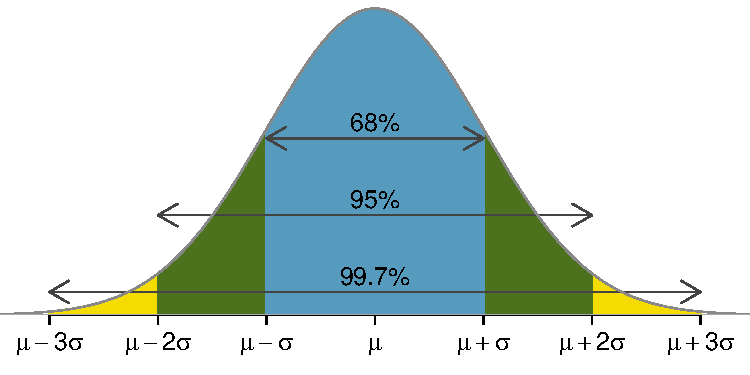
\includegraphics[width=0.72\textwidth]{ch_distributions/figures/6895997/6895997}
\caption{Probabilities for falling within 1, 2, and 3 standard deviations of the mean in a normal distribution.}
\label{6895997}
\end{figure}

\begin{exercisewrap}
\begin{nexercise}
Use the Z table to confirm that about 68\%, 95\%, and 99.7\% of observations fall within 1, 2, and 3, standard deviations of the mean in the normal distribution, respectively. For instance, first find the area that falls between $Z=-1$ and $Z=1$, which should have an area of about 0.68. Similarly there should be an area of about 0.95 between $Z=-2$ and $Z=2$.\footnotemark\end{nexercise}
\end{exercisewrap}
\footnotetext{First draw the pictures. To find the area between $Z=-1$ and $Z=1$, use the normal probability table to determine the areas below $Z=-1$ and above $Z=1$. Next verify the area between $Z=-1$ and $Z=1$ is about 0.68. Repeat this for $Z=-2$ to $Z=2$ and also for $Z=-3$ to $Z=3$.}

It is possible for a normal random variable to fall 4,~5, or~even more standard deviations from the mean. However, these occurrences are very rare if the data are nearly normal. The probability of being further than 4 standard deviations from the mean is about 1-in-15,000. For 5 and 6 standard deviations, it is about 1-in-2 million and 1-in-500 million, respectively.

\begin{exercisewrap}
\begin{nexercise}
SAT scores closely follow the normal model with mean $\mu = 1100$ and standard deviation $\sigma = 200$. (a) About what percent of test takers score 700 to 1500? (b) What percent score between 1100 and 1500?\footnotemark
\end{nexercise}
\end{exercisewrap}
\footnotetext{(a) 700 and 1500 represent two standard deviations above and below the mean, which means about 95\% of test takers will score between 700 and 1500. (b)~Since the normal model is symmetric, then half of the test takers from part~(a) ($\frac{95\%}{2} = 47.5\%$ of all test takers) will score 700 to 1500 while 47.5\% score between 1100 and 1500.}


\D{\newpage}

%%
\subsection{Evaluating the normal approximation}
\label{assessingNormal}

It is important to remember normality is always an approximation. Testing the appropriateness of the normal assumption is a key step in many data analyses.

%\index{normal probability plot|(}

The distribution of heights of US males is well approximated by the normal model. We are interested in proceeding under the assumption that the data are normally distributed, but first we must check to see if this is reasonable.

There are two visual methods for checking the assumption of normality that can be implemented and interpreted quickly. The first is a simple histogram with the best fitting normal curve overlaid on the plot, as shown in the left panel of Figure~\ref{fcidMHeights}. The sample mean $\bar{x}$ and standard deviation $s$ are used as the parameters of the best fitting normal curve. The closer this curve fits the histogram, the more reasonable the normal model assumption. Another more common method is examining a \term{normal probability plot},\footnote{Also commonly called a \term{quantile-quantile plot}.} shown in the right panel of Figure~\ref{fcidMHeights}. The closer the points are to a perfect straight line, the more confident we can be that the data follow the normal model.

\begin{figure}[ht]
\centering
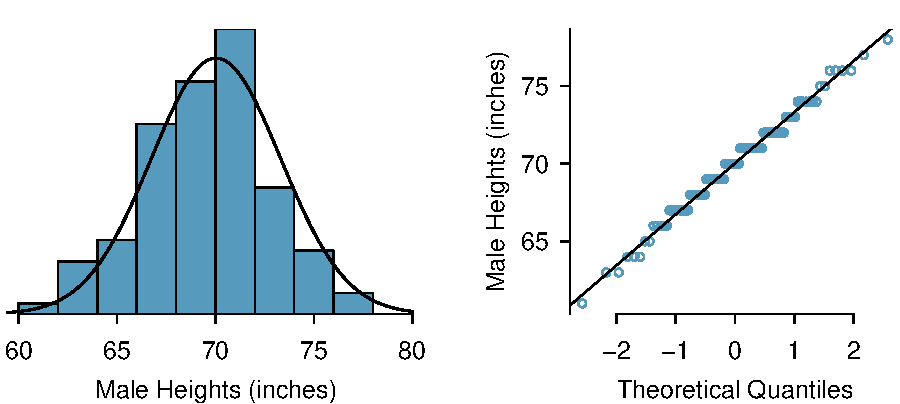
\includegraphics[width=0.78\textwidth]{ch_distributions/figures/fcidMHeights/fcidMHeights}
\caption{A sample of 100 male heights. The observations are rounded to the nearest whole inch, explaining why the points appear to jump in increments in the normal probability plot.}
\label{fcidMHeights}
\end{figure}


Three data sets of 40, 100, and 400 samples were simulated from a normal distribution, and the histograms and normal probability plots of the data sets are shown in Figure~\ref{normalExamples}. These will provide a benchmark for what to look for in plots of real data. \label{normalExamplesExample}

\begin{figure}
\centering
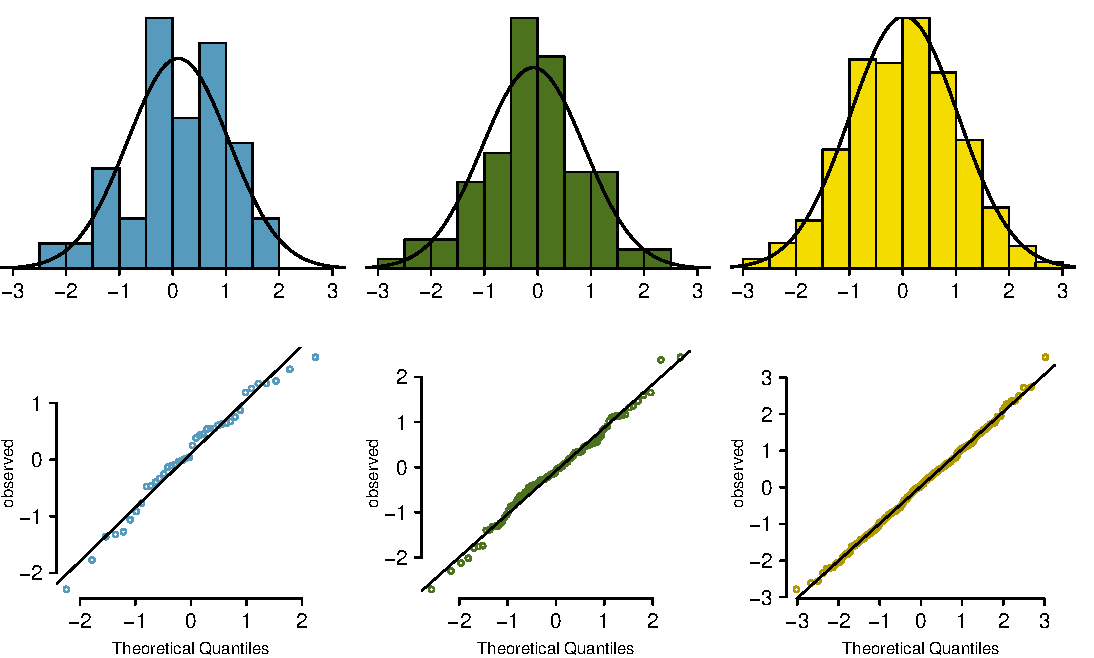
\includegraphics[width=\textwidth]{ch_distributions/figures/normalExamples/normalExamples}
\caption{Histograms and normal probability plots for three simulated normal data sets; $n=40$ (left), $n=100$ (middle), $n=400$ (right).}
\label{normalExamples}
\end{figure}

The left panels show the histogram (top) and normal probability plot (bottom) for the simulated data set with 40 observations. The data set is too small to really see clear structure in the histogram. The normal probability plot also reflects this, where there are some deviations from the line. However, these deviations are not strong.

The middle panels show diagnostic plots for the data set with 100 simulated observations. The histogram shows more normality and the normal probability plot shows a better fit. While there is one observation that deviates noticeably from the line, it is not particularly extreme.

The data set with 400 observations has a histogram that greatly resembles the normal distribution, while the normal probability plot is nearly a perfect straight line. Again in the normal probability plot there is one observation (the largest) that deviates slightly from the line. If that observation had deviated 3 times further from the line, it would be of much greater concern in a real data set. Apparent outliers can occur in normally distributed data but they are rare.

Notice the histograms look more normal as the sample size increases, and the normal probability plot becomes straighter and more stable.


\begin{examplewrap}
\begin{nexample}{Consider all NBA players from the 2018-2019 season presented in Figure~\ref{nbaNormal}.\footnotemark\,  Based on the graphs, are NBA player heights normally distributed? }
We first create a histogram and normal probability plot of the NBA player heights. The histogram in the left panel is slightly left skewed, which contrasts with the symmetric normal distribution. The points in the normal probability plot do not appear to closely follow a straight line but show what appears to be a ``wave''. We can compare these characteristics to the sample of 400 normally distributed observations in Example~\ref{normalExamplesExample} and see that they represent much stronger deviations from the normal model. NBA player heights do not appear to come from a normal distribution.
\end{nexample}
\end{examplewrap}
\footnotetext{These data were collected from \oiRedirect{textbook-nba_com}{www.nba.com}.}

\begin{figure}
\centering
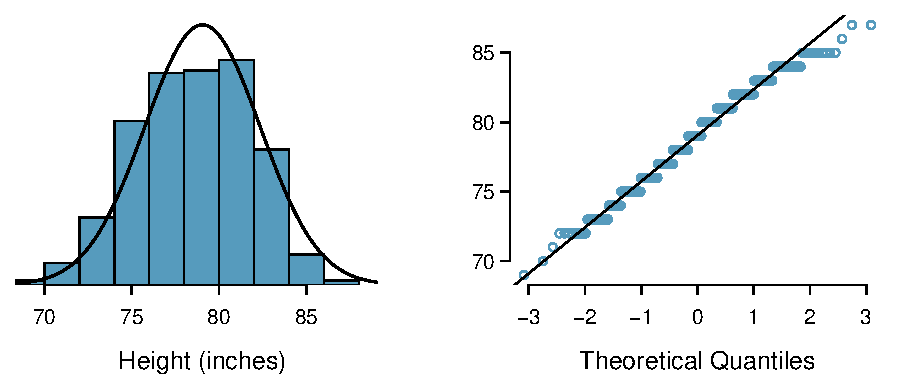
\includegraphics[width=0.9\textwidth]{ch_distributions/figures/nbaNormal/nbaNormal}
\caption{Histogram and normal probability plot for the NBA heights from the 2018-2019 season.}
\label{nbaNormal}
\end{figure}

\begin{examplewrap}
\begin{nexample}{Consider the poker winnings of an individual over 50 days.  A histogram and normal probability plot of these data are shown in Figure~\ref{pokerNormal}. Based on the graphs, can we approximate poker winnings by a normal distribution?} 
The data are very strongly right skewed\index{skew!example: very strong} in the histogram, which corresponds to the very strong deviations on the upper right component of the normal probability plot. If we compare these results to the sample of 40 normal observations in Example~\ref{normalExamplesExample}, it is apparent that these data show very strong deviations from the normal model.
\end{nexample}
\end{examplewrap}

\begin{figure}
\centering
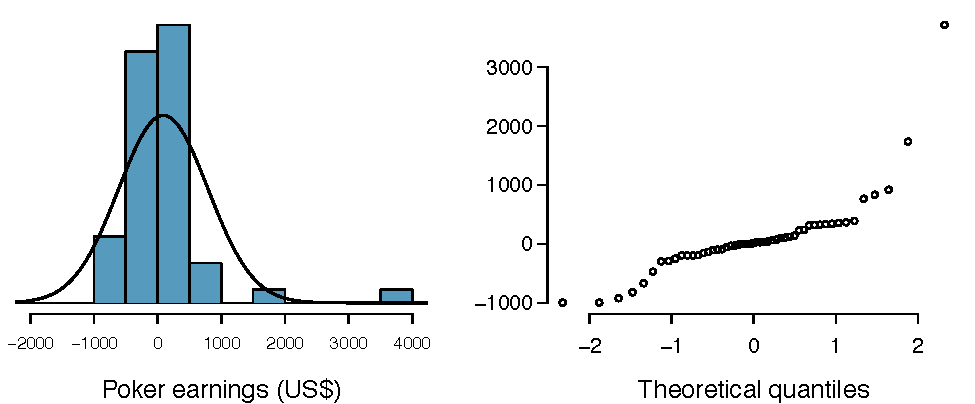
\includegraphics[width=0.9\textwidth]{ch_distributions/figures/pokerNormal/pokerNormal}
\caption{A histogram of poker data with the best fitting normal plot and a normal probability plot.}
\label{pokerNormal}
\end{figure}

\D{\newpage}

\begin{exercisewrap}
\begin{nexercise}\label{normalQuantileExercise}%
Determine which data sets represented in Figure~\ref{normalQuantileExer} plausibly come from a nearly normal distribution. Are you confident in all of your conclusions? There are 100 (top left), 50 (top right), 500 (bottom left), and 15 points (bottom right) in the four plots.\footnotemark
\end{nexercise}
\end{exercisewrap}
\footnotetext{Answers may vary a little. The top-left plot shows some deviations in the smallest values in the data set; specifically, the left tail of the data set has some outliers we should be wary of. The top-right and bottom-left plots do not show any obvious or extreme deviations from the lines for their respective sample sizes, so a normal model would be reasonable for these data sets. The bottom-right plot has a consistent curvature that suggests it is not from the normal distribution. If we examine just the vertical coordinates of these observations, we see that there is a lot of data between -20 and 0, and then about five observations scattered between 0 and 70. This describes a distribution that has a strong right skew.}

\begin{figure}[h]
\centering
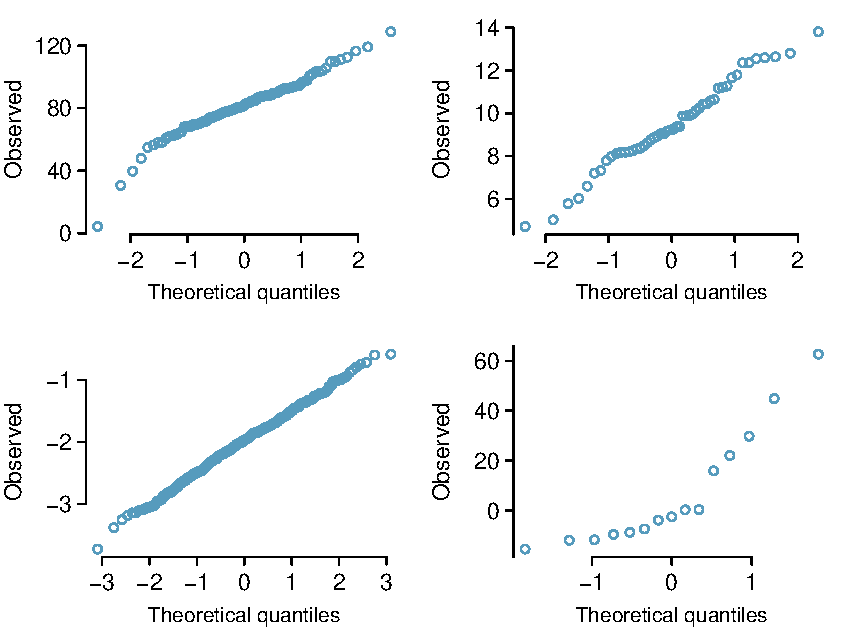
\includegraphics[width=0.75\textwidth]{ch_distributions/figures/normalQuantileExer/normalQuantileExer}
\caption{Four normal probability plots for Guided Practice~\ref{normalQuantileExercise}.}
\label{normalQuantileExer}
\end{figure}

\begin{exercisewrap}
\begin{nexercise} \label{normalQuantileExerciseAdditional}
Figure~\ref{normalQuantileExerAdditional} shows normal probability plots for two distributions that are skewed. One distribution is skewed to the low end (left skewed) and the other to the high end (right skewed). Which is which?\footnotemark
\end{nexercise}
\end{exercisewrap}
\footnotetext{Examine where the points fall along the vertical axis. In the first plot, most points are near the low end with fewer observations scattered along the high end; this describes a distribution that is skewed to the high end. The second plot shows the opposite features, and this distribution is skewed to the low end.}

\begin{figure}[h]
\centering
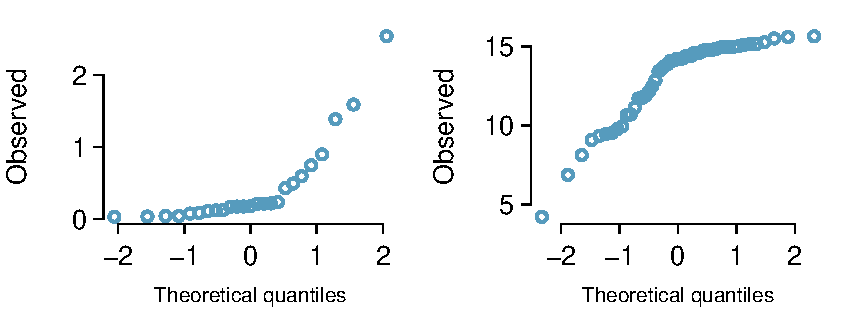
\includegraphics[width=0.75\textwidth]{ch_distributions/figures/normalQuantileExer/normalQuantileExerAdditional}
\caption{Normal probability plots for Guided Practice~\ref{normalQuantileExerciseAdditional}.}
\label{normalQuantileExerAdditional}
\end{figure}



%%
%%
\subsection{Normal approximation for sums of random variables}
\label{normapproxsumrv}

We have seen that many distributions are approximately normal. The sum and the difference of normally distributed variables is also normal. While we cannot prove this here, the usefulness of it is seen in the following example.

\begin{examplewrap}
\begin{nexample}{Three friends are playing a cooperative video game in which they have to complete a puzzle as fast as possible. Assume that the individual times of the 3 friends are independent of each other. The individual times of the friends in similar puzzles are approximately normally distributed with the following means and standard deviations. 
\begin{center}
\begin{tabular}{lrr}
& Mean &  SD \\
Friend 1 	& 5.6 & 0.11  \\
Friend 2 	& 5.8  & 0.13 \\
Friend 3 	& 6.1  & 0.12  
\end{tabular}
\end{center}
To advance to the next level of the game, the friends' total time must not exceed 17.1 minutes. What is the probability that they will advance to the next level?}
Because each friend's time is approximately normally distributed, \emph{the sum of their times is also approximately normally distributed}. We will do a normal approximation, but first we need to find the mean and standard deviation of the \emph{sum}. We learned how to do this in Section~\ref{randomVariablesSection}.

Let the three friends be labeled $X$, $Y$, $Z$. We want $P(X + Y + Z < 17.1)$. The mean and standard deviation of the sum of $X$, $Y$, and $Z$ is given by:
\begin{align*}
\mu_{sum} &= E(X+Y+Z)
	& \sigma_{sum}&= \sqrt{(SD_X)^2+(SD_Y)^2 + (SD_Z)^2} \\
&= E(X) + E(Y) + E(Z)
	& &= \sqrt{(0.11)^2+(0.13)^2+(0.12)^2}\\
&=5.6+5.8+6.1
	& &= 0.208 \\
&=17.5
\end{align*}
Now we can find the Z-score. 
\begin{align*}
Z &= \frac{x_{sum}-\mu_{sum}}{\sigma_{sum}} \\
&=\frac{17.1-17.5}{0.208} \\
&=-1.92
\end{align*}
Finally, we want the probability that the sum is less than 17.5, so we shade the area to the left of $Z = -1.92$. Using the normal table or a calculator, we get
\begin{align*}
P(Z < -1.92) = 0.027
\end{align*}
There is a 2.7\% chance that the friends will advance to the next level.
\end{nexample}
\end{examplewrap}

\begin{exercisewrap}
\begin{nexercise}
What is the probability that Friend 2 will complete the puzzle with a faster time than Friend 1?  Hint:  find $P(Y < X)$, or $P(Y - X < 0)$.\footnotemark
\end{nexercise}
\end{exercisewrap}
\footnotetext{First find the mean and standard deviation of $Y - X$. The mean of $Y - X$ is $\mu_{Y-X} = 5.8 - 5.6 =  0.2$. The standard deviation is  $SD_{Y-X}=\sqrt{(0.13)^2+(0.11)^2}=0.170$. Then $Z=\frac{0-0.2}{0.170}=-1.18$ and $P(Z < -1.18)= .119$. There is an 11.9\% chance that Friend 2 will complete the puzzle with a faster time than Friend 1.}


\D{\newpage}

%%
\subsection*{Section summary}

\begin{itemize}
\item A \term{Z-score} represents the number of standard deviations a value in a data set is above or below the mean.  To calculate a \mbox{Z-score} use: $Z = \frac{x-\text{mean}}{SD}$.  

\item \emph{Z-scores do not depend on units}.  When looking at distributions with different units or different standard deviations, \mbox{Z-scores} are useful for comparing how far values are away from the mean (relative to the distribution of the data). 

\item The \term{normal distribution} is the most commonly used distribution in Statistics.  Many distribution are approximately normal, but none are exactly normal.  

\item The empirical rule (68-95-99.7 Rule) comes from the normal distribution.  The closer a distribution is to normal, the better this rule will hold.

\item It is often useful to use the standard normal distribution, which has mean~0 and SD~1, to approximate a discrete histogram.  There are two common types of \textbf{normal approximation problems}, and for each a key step is to find a \mbox{Z-score}.   
\begin{itemize}
\item[A:] \textit{Find the percent or probability of a value greater/less than a given \textit{x}-value.  }
\begin{enumerate}\vspace{-1mm}
\setlength{\itemsep}{0mm}
\item Verify that the distribution of interest is approximately normal.
\item Calculate the \mbox{Z-score}.  Use the provided population mean and SD to standardize the given $x$-value.
\item Use a calculator function (e.g. \calctext{normcdf} on a TI) or a normal table to find the area under the normal curve to the right/left of this \mbox{Z-score}; this is the \textit{estimate} for the percent/probability.
\end{enumerate}

\item[B:] \textit{Find the \textit{x}-value that corresponds to a given percentile.}
\begin{enumerate}\vspace{-1mm}
\setlength{\itemsep}{0mm}
\item Verify that the distribution of interest is approximately normal.
\item Find the Z-score that corresponds to the given percentile (using, for example, \calctext{invNorm} on a TI).  
\item Use the Z-score along with the given mean and SD to solve for the \textit{x}-value.  
\end{enumerate}
\end{itemize}

\item Because the sum or difference of two normally distributed variables is itself a normally distributed variable, the normal approximation is also used in the following type of problem.
\item[] \textit{Find the probability that a sum $X+Y$ or a difference $X-Y$ is greater/less than some value}.
\begin{enumerate}\vspace{-1mm}
\setlength{\itemsep}{0mm}
\item Verify that the distribution of $X$ and the distribution of $Y$ are approximately normal.  
\item Find the mean of the sum or difference.  Recall: the mean of a sum is the 
\\sum of the means.  The mean of a difference is the difference of the means.  
\\Find the SD of the sum or difference using:  
\\$SD(X+Y) = SD(X - Y) =  \sqrt{(SD(X))^2 + (SD(Y))^2}$.
\item Calculate the Z-score.  Use the calculated mean and SD to standardize the given sum or difference.
\item Find the appropriate area under the normal curve. 
\end{enumerate}


\end{itemize}

%%%%%%%%Section exercises
{\exercisesheader{}

% 1

\eoce{\qt{Area under the curve, Part I\label{area_under_curve_1}} What percent of a 
standard normal distribution $N(\mu=0, \sigma=1)$ is found in each region? 
Be sure to draw a graph. \vspace{-3mm}
\begin{multicols}{4}
\begin{parts}
\item $Z < -1.35$
\item $Z > 1.48$
\item $-0.4 < Z < 1.5$
\item $|Z| > 2$
\end{parts}
\end{multicols}
}{}

% 2

\eoce{\qt{Area under the curve, Part II\label{area_under_curve_2}} What percent of 
a standard normal distribution $N(\mu=0, \sigma=1)$ is found in each region? 
Be sure to draw a graph. \vspace{-3mm}
\begin{multicols}{4}
\begin{parts}
\item $Z > -1.13$
\item $Z < 0.18$
\item $Z > 8$
\item $|Z| < 0.5$
\end{parts}
\end{multicols}
}{}

% 3

\eoce{\qt{GRE scores, Part I\label{GRE_intro}} Sophia who took the Graduate Record 
Examination (GRE) scored 160 on the Verbal Reasoning section and 157 on the 
Quantitative Reasoning section. The mean score for Verbal Reasoning section 
for all test takers was 151 with a standard deviation of 7, and the mean 
score for the Quantitative Reasoning was 153 with a standard deviation of 
7.67. Suppose that both distributions are nearly normal. 
\begin{parts}
\item What is  Sophia's Z-score on the Verbal Reasoning section? On the 
Quantitative Reasoning section? Draw a standard normal distribution curve and 
mark these two Z-scores.
\item What do these Z-scores tell you?
\item Relative to others, which section did she do better on?
\item Find her percentile scores for the two exams.
\item What percent of the test takers did better than her on the Verbal 
Reasoning section? On the Quantitative Reasoning section?
\item Explain why simply comparing raw scores from the two sections could lead 
to an incorrect conclusion as to which section a student did better on.
\item If the distributions of the scores on these exams are not nearly 
normal, would your answers to parts (b) - (e) change? Explain your reasoning.
\end{parts}
}{}

% 4

\eoce{\qt{Triathlon times, Part I\label{triathlon_times_intro}} In triathlons, it 
is common for racers to be placed into age and gender groups. Friends Leo and 
Mary both completed the Hermosa Beach Triathlon, where Leo competed in the 
\textit{Men, Ages 30 - 34} group while Mary competed in the \textit{Women, 
Ages 25 - 29} group. Leo completed the race in 1:22:28 (4948 seconds), while 
Mary completed the race in 1:31:53 (5513 seconds). Obviously Leo finished 
faster, but they are curious about how they did within their respective 
groups. Can you help them? Here is some information on the performance of 
their groups:
\begin{itemize}
\setlength{\itemsep}{0mm}
\item The finishing times of the \textit{Men, Ages 30 - 34} group has a mean 
of 4313 seconds with a standard deviation of 583 seconds.
\item The finishing times of the \textit{Women, Ages 25 - 29} group has a 
mean of 5261 seconds with a standard deviation of 807 seconds.
\item The distributions of finishing times for both groups are approximately 
Normal.
\end{itemize}
Remember: a better performance corresponds to a faster finish.
\begin{parts}
\item What are the Z-scores for Leo's and Mary's finishing times? What do 
these Z-scores tell you?
\item Did Leo or Mary rank better in their respective groups? Explain your 
reasoning.
\item What percent of the triathletes did Leo finish faster than in his group?
\item What percent of the triathletes did Mary finish faster than in her 
group?
\item If the distributions of finishing times are not nearly normal, would 
your answers to parts (a)~-~(d) change? Explain your reasoning.
\end{parts}
}{}

% 5

\eoce{\qt{GRE scores, Part II\label{GRE_cutoffs}} In Exercise~\ref{GRE_intro} we 
saw two distributions for GRE scores: $N(\mu=151, \sigma=7)$ for the verbal 
part of the exam and $N(\mu=153, \sigma=7.67)$ for the quantitative part. Use 
this information to compute each of the following:
\begin{parts}
\item The score of a student who scored in the $80^{th}$ percentile on the 
Quantitative Reasoning section.
\item The score of a student who scored worse than 70\% of the test takers in 
the Verbal Reasoning section.
\end{parts}
}{}

\D{\newpage}

% 6

\eoce{\qt{Triathlon times, Part II\label{triathlon_times_cutoffs}} In 
Exercise~\ref{triathlon_times_intro} we saw two distributions for triathlon 
times: $N(\mu=4313, \sigma=583)$ for \emph{Men, Ages 30 - 34} and 
$N(\mu=5261, \sigma=807)$ for the \emph{Women, Ages 25 - 29} group. Times are 
listed in seconds. Use this information to compute each of the following:
\begin{parts}
\item The cutoff time for the fastest 5\% of athletes in the men's group, i.e. those 
who took the shortest 5\% of time to finish. 
\item The cutoff time for the slowest 10\% of athletes in the women's group. 
\end{parts}
}{}

% 7

\eoce{\qt{LA weather, Part I\label{la_weather_intro}} \videohref{ahss_eoce_sol-la_weather_intro}\ \ The average daily high 
temperature in June in LA is 77\degree F with a standard deviation of 
5\degree F. Suppose that the temperatures in June closely follow a normal 
distribution. 
\begin{parts}
\item What is the probability of observing an 83\degree F temperature or 
higher in LA during a randomly chosen day in June?
\item How cool are the coldest 10\% of the days (days with lowest average 
high temperature) during June in LA?
\end{parts}
}{}

% 8

\eoce{\qt{CAPM\label{CAPM}} The Capital Asset Pricing Model (CAPM) is a financial 
model that assumes returns on a portfolio are normally distributed. Suppose a 
portfolio has an average annual return of 14.7\% (i.e. an average gain of 
14.7\%) with a standard deviation of 33\%. A return of 0\% means the value of 
the portfolio doesn't change, a negative return means that the portfolio 
loses money, and a positive return means that the portfolio gains money.
\begin{parts}
\item What percent of years does this portfolio lose money, i.e. have a 
return less than 0\%?
\item What is the cutoff for the highest 15\% of annual returns with this 
portfolio?
\end{parts}
}{}

% 9

\eoce{\qt{LA weather, Part II\label{la_weather_unit_change}} 
Exercise~\ref{la_weather_intro} states that average daily high temperature in 
June in LA is 77\degree F with a standard deviation of 5\degree F, and it can 
be assumed that they to follow a normal distribution. We use the following 
equation to convert \degree F (Fahrenheit) to \degree C (Celsius):
\[ C = (F - 32) \times \frac{5}{9}. \]
\begin{parts}
\item What is the probability of observing a 28\degree C (which roughly 
corresponds to 83\degree F) temperature or higher in June in LA? Calculate 
using the \degree C model from part (a).
\item Did you get the same answer or different answers in part (b) of this 
question and part (a) of Exercise~\ref{la_weather_intro}? Are you surprised? Explain.
\item Estimate the IQR of the temperatures (in \degree C) in June in LA.
\end{parts}
}{}

% 10

\eoce{\qt{Find the SD\label{find_sd}} Cholesterol levels for women aged 20 to 34 follow an approximately 
normal distribution with mean 185 milligrams per deciliter (mg/dl). Women 
with cholesterol levels above 220 mg/dl are considered to have high 
cholesterol and about 18.5\% of women fall into this category.  Find the standard deviation of this distribution.
}{}


% 11

\eoce{\qt{Scores on stats final, Part I} \label{statsScores} Below are final exam scores of 20 Introductory Statistics students. 
\[ \stackrel{1}{57}, \stackrel{2}{66}, \stackrel{3}{69}, \stackrel{4}{71}, \stackrel{5}{72}, \stackrel{6}{73}, \stackrel{7}{74}, \stackrel{8}{77}, \stackrel{9}{78}, \stackrel{10}{78}, \stackrel{11}{79}, \stackrel{12}{79}, \stackrel{13}{81}, \stackrel{14}{81}, \stackrel{15}{82}, \stackrel{16}{83}, \stackrel{17}{83}, \stackrel{18}{88}, \stackrel{19}{89}, \stackrel{20}{94} \]
The mean score is 77.7 points. with a standard deviation of 8.44 points. Use this information to determine if the scores approximately follow the 68-95-99.7\% Rule.
}{}

% 12

\eoce{\qt{Heights of female college students, Part I} \label{collegeFemHeights} Below are heights of 25 female college students.
\[ \stackrel{1}{54}, \stackrel{2}{55}, \stackrel{3}{56}, \stackrel{4}{56}, \stackrel{5}{57}, \stackrel{6}{58}, \stackrel{7}{58}, \stackrel{8}{59}, \stackrel{9}{60}, \stackrel{10}{60}, \stackrel{11}{60}, \stackrel{12}{61}, \stackrel{13}{61}, \stackrel{14}{62}, \stackrel{15}{62}, \stackrel{16}{63}, \stackrel{17}{63}, \stackrel{18}{63}, \stackrel{19}{64}, \stackrel{20}{65}, \stackrel{21}{65}, \stackrel{22}{67}, \stackrel{23}{67}, \stackrel{24}{69}, \stackrel{25}{73} \]
The mean height is 61.52 inches with a standard deviation of 4.58 inches. Use this information to determine if the heights approximately follow the 68-95-99.7\% Rule.
}{}

\D{\newpage}


% 13

\eoce{\qt{Lemonade at The Cafe} Drink pitchers at The Cafe are intended to hold about 64 ounces of lemonade and glasses hold about 12 ounces. However, when the pitchers are filled by a server, they do not always fill it with exactly 64 ounces. There is some variability. Similarly, when they pour out some of the lemonade, they do not pour exactly 12 ounces. The amount of lemonade in a pitcher is normally distributed with mean 64 ounces and standard deviation 1.732 ounces. The amount of lemonade in a glass is normally distributed with mean 12 ounces and standard deviation 1 ounce. 
\begin{parts}
\item How much lemonade would you expect to be left in a pitcher after pouring one glass of lemonade? 
\item What is the standard deviation of the amount left in a pitcher after pouring one glass of lemonade? 
\item What is the probability that more than 50 ounces of lemonade is left in a pitcher after pouring one glass of lemonade?
\end{parts}
}{}

% 14

\eoce{\qt{Spray paint, Part I} \label{sprayPaint} Suppose the area that can be painted using a single can of spray paint is slightly variable and follows a nearly normal distribution with a mean of 25 square feet and a standard deviation of 3 square feet. Suppose also that you buy three cans of spray paint.
\begin{parts}
\item How much area would you expect to cover with these three cans of spray paint?
\item What is the standard deviation of the area you expect to cover with these three cans of spray paint?
\item The area you wanted to cover is 80 square feet. What is the probability that you will be able to cover this entire area with these three cans of spray paint?
\end{parts}
}{}

% 15

\eoce{\qt{GRE scores, Part III\label{GRE_scores_3}} \videohref{ahss_eoce_sol-gre_scores_part_III}\ \ 
In Exercises~\ref{GRE_intro} and~\ref{GRE_cutoffs} we saw two distributions for GRE scores: $N(\mu=151, \sigma=7)$ for the verbal part of the exam and $N(\mu=153, \sigma=7.67)$ for the quantitative part. Suppose performance on these two sections is independent. Use this information to compute each of the following:
\begin{parts}
\item The probability of a combined (verbal + quantitative) score above 320. 
\item The score of a student who scored better than 90\% of the test takers overall.
\end{parts}
}{}

% 16
\eoce{\qt{Betting on dinner, Part I} \label{dinnerBet} Suppose a restaurant is running a promotion where prices of menu items are random following some underlying distribution. If you're lucky, you can get a basket of fries for \$3, or if you're not so lucky you might end up having to pay \$10 for the same menu item. The price of basket of fries is drawn from a normal distribution with mean \$6 and standard deviation of \$2. The price of a fountain drink is drawn from a normal distribution with mean \$3 and standard deviation of \$1. What is the probability that you pay more than \$10 for a dinner consisting of a basket of fries and a fountain drink?}
{}

}


%____________________________________
\section[Sampling distribution of a sample mean]{Sampling distribution of a sample mean }
\label{distributionofxbar}

\sectionintro{
\noindent%
If bags of chips are produced with an average weight of 15~oz and a standard deviation of 0.1~oz, what is the probability that the average weight of 30 bags will be within 0.1~oz of the mean?  The answer is not 68\%!
To answer this question we must visualize and understand what is called the \emph{sampling distribution} of a sample mean.


%%
\subsection*{Learning objectives}
\begin{enumerate}
\setlength{\itemsep}{0mm}
\item Understand the concept of a sampling distribution.

\item Describe the center, spread, and shape of the sampling distribution of a sample mean.


\item Distinguish between the standard deviation of a population and the standard deviation of a sampling distribution.

\item Explain the content and importance of the Central Limit Theorem.

\item Identify and explain the conditions for using normal approximation involving a sample mean.

\item Verify that the conditions for normal approximation are met and carry out normal approximation involving a sample mean or sample sum.

\end{enumerate}
}


%%
\subsection[The mean and standard deviation of $\bar{x}$]{The mean and standard deviation of $\pmb{\bar{x}}$}


In this section we consider a data set called \data{run17}, which represents all 19,961 runners who finished the 2017 Cherry Blossom 10 mile run in Washington, DC.\footnote{\oiRedirect{textbook-cherryblossom_org}{www.cherryblossom.org}} Part of this data set is shown in Figure~\ref{run17DF}, and the variables are described in Figure~\ref{run17Variables}.

\begin{figure}[h]
\centering
\begin{tabular}{rrrrr}
  \hline
ID & time & age & gender & state \\ 
  \hline
1 & 92.25 & 38.00 & M & MD \\ 
2 & 106.35 & 33.00 & M & DC \\ 
%3 & 89.33 & 55.00 & F & VA \\ 
%4 & 113.50 & 24.00 & F & VA \\ 
$\vdots$ & $\vdots$ & $\vdots$ & $\vdots$ & $\vdots$ \\
16923 & 122.87 & 37.00 & F & VA \\ 
16924 & 93.30 & 27.00 & F & DC \\ 
   \hline
\end{tabular}
\caption{Four observations from the \data{run17} data set.}
\label{run17DF}
\end{figure}
% library(openintro); library(xtable); data(run10); xtable(run10[c(1,2,3,4, nrow(run10)-1:0), c("time", "age", "gender", "state")])

\begin{figure}[h]
\centering\small
\begin{tabular}{l p{65mm}}
\hline
{\bf variable} & {\bf description} \\
\hline
\var{time} & Ten mile run time, in minutes \\
\var{age} & Age, in years \\
\var{gender} & Gender (\resp{M} for male, \resp{F} for female) \\
\var{state} & Home state (or country if not from the US) \\
\hline
\end{tabular}
\caption{Variables and their descriptions for the \data{run17} data set.}
\label{run17Variables}
\end{figure}

\index{data!run17samp|(}

These data are special because they include the results for the entire population of runners who finished the 2017 Cherry Blossom Run. We took a simple random sample of this population, which is represented in Figure~\ref{run17sampDF}. A histogram summarizing the time variable in the \data{run17samp} data set is shown in Figure~\ref{run17sampHistograms}.

\begin{figure}[h]
\centering
\begin{tabular}{rrrrr}
  \hline
ID & time & age & gender & state \\ 
  \hline
1983 & 88.31 & 59 & M & MD \\ 
8192 & 100.67 & 32 & M & VA \\ 
%11020 & 109.52 & 33 & F & VA \\ 
  $\vdots$ &   $\vdots$ &   $\vdots$ &   $\vdots$ &   $\vdots$ \\ 
1287 & 89.49 & 26 & M & DC \\ 
   \hline
\end{tabular}
\caption{Three observations for the \data{run17samp} data set, which represents a simple random sample of 100 runners from the 2017 Cherry Blossom Run.}
\label{run17sampDF}
%library(openintro); library(xtable); data(run10); data(run10samp); xtable(run10samp[c(1,2,3,100),])
\end{figure}

% WARNING: This figure is referenced in Section 4.2

\begin{figure}[h]
\centering
\includegraphics[width=0.75\textwidth]{ch_distributions/figures/run17sampHistograms/run17sampHistograms} 
\caption{Histogram of \var{time} for a single sample of size 100. The average of the sample is in the mid-90s and the standard deviation of the sample $s\approx 17$ minutes.
\index{skew!example: moderate}}
\label{run17sampHistograms}
\end{figure}

From the random sample represented in \data{run17samp}, we guessed the average time it takes to run 10 miles is 95.61 minutes. Suppose we take another random sample of 100 individuals and take its mean: 95.30 minutes. Suppose we took another (93.43 minutes) and another (94.16 minutes), and so on. If we do this many many times -- which we can do only because we have the entire population data set -- we can build up a \term{sampling distribution} for the sample mean when the sample size is 100, shown in Figure~\ref{netTime1000SamplingDistribution}.

\begin{figure}[h]
   \centering
   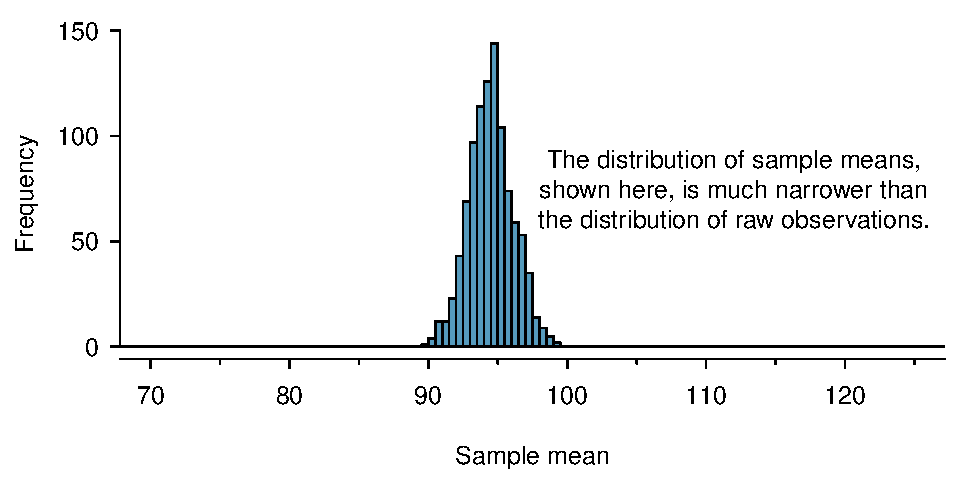
\includegraphics[width=\textwidth]{ch_distributions/figures/netTime1000SamplingDistribution/netTime1000SamplingDistribution}
   \caption{A histogram of 1000 sample means for run time, where the samples are of size $n=100$. This histogram approximates the true sampling distribution of the sample mean, with mean $\mu_{\bar{x}}$ and standard deviation $\sigma_{\bar{x}}$.}
   \label{netTime1000SamplingDistribution}
\end{figure}

\begin{onebox}{Sampling distribution}
The sampling distribution represents the distribution of the point estimates based on samples of a fixed size from a certain population. It is useful to think of a point estimate as being drawn from such a distribution. Understanding the concept of a sampling distribution is central to understanding statistical inference.\end{onebox}


The sampling distribution shown in Figure~\ref{netTime1000SamplingDistribution} is unimodal and approximately symmetric. It is also centered exactly at the true population mean: $\mu=94.52$. Intuitively, this makes sense. The sample mean should be an unbiased estimator of the population mean. Because we are considering the distribution of the sample mean, we will use $\mu_{\bar{x}} = 94.52$ to describe the true mean of this distribution.

\D{\newpage}

We can see that the sample mean has some variability around the population mean, which can be quantified using the standard deviation of this distribution of sample means. The standard deviation of the sample mean tells us how far the typical estimate is away from the actual population mean, 94.52 minutes. It also describes the typical \term{error} of a single estimate, and is denoted by the symbol $\sigma_{\bar{x}}$. 

\begin{onebox}{Standard deviation of an estimate}
The standard deviation associated with an estimate describes the typical error or uncertainty associated with the estimate.\end{onebox}

\begin{examplewrap}
\begin{nexample}{Looking at Figures~\ref{run17sampHistograms} and \ref{netTime1000SamplingDistribution}, we see that the standard deviation of the sample mean with $n=100$ is much smaller than the standard deviation of a single sample. Interpret this statement and explain why it is true.}The variation from one sample mean to another sample mean is much smaller than the variation from one individual to another individual. This makes sense because when we average over 100 values, the large and small values tend to cancel each other out. While many individuals have a time under 90 minutes, it would be unlikely for the \emph{average} of 100 runners to be less than 90 minutes.
\end{nexample}
\end{examplewrap}

\D{\newpage}

\begin{exercisewrap}
\begin{nexercise}
(a) Would you rather use a small sample or a large sample when estimating a parameter? Why? (b) Using your reasoning from (a), would you expect a point estimate based on a small sample to have smaller or larger standard deviation than a point estimate based on a larger sample?\footnotemark
\end{nexercise}
\end{exercisewrap}
\footnotetext{(a) Consider two random samples: one of size 10 and one of size 1000. Individual observations in the small sample are highly influential on the estimate while in larger samples these individual observations would more often average each other out. The larger sample would tend to provide a more accurate estimate. (b) If we think an estimate is better, we probably mean it typically has less error. Based on (a), our intuition suggests that a larger sample size corresponds to a smaller standard deviation.}

When considering how to calculate the standard deviation of a sample mean, there is one problem: there is no obvious way to estimate this from a single sample. However, statistical theory provides a helpful tool to address this issue.

In the sample of 100 runners, the standard deviation of the sample mean is equal to one-tenth of the population standard deviation: $15.93/10 = 1.59$. In other words, the standard deviation of the sample mean based on 100 observations is equal to
\begin{eqnarray*}
SD_{\bar{x}} = \sigma_{\bar{x}} = \frac{\sigma_{x}}{\sqrt{n}} = \frac{15.93}{\sqrt{100}} = 1.59
\end{eqnarray*}
where $\sigma_{x}$ is the standard deviation of the individual observations. This is no coincidence. We can show mathematically that this equation is correct when the observations are independent  using the probability tools of Section~\ref{randomVariablesSection}.

\D{\newpage}

\begin{onebox}{Computing SD for the sample mean}
Given $n$ independent observations from a population with standard deviation $\sigma$, the standard deviation of the sample mean is equal to \vspace{-1mm}
\begin{eqnarray}
SD_{\bar{x}} = \sigma_{\bar{x}} =  \frac{\sigma}{\sqrt{n}}
\label{seOfXBar}
\end{eqnarray}\vspace{-3mm}

A reliable method to ensure sample observations are independent is to conduct a simple random sample consisting of less than 10\% of the population.\index{standard error!single mean}\end{onebox}

\begin{exercisewrap}
\begin{nexercise}
The average of the runners' ages is 35.05 years with a standard deviation of $\sigma = 8.97$. A simple random sample of 100 runners is taken. (a)~What is the standard deviation of the sample mean? (b)~Would you be surprised to get a sample of size 100 with an average of 36~years?\footnotemark\end{nexercise}
\end{exercisewrap}
\footnotetext{(a) Use Equation~(\ref{seOfXBar}) with the population standard deviation to compute the standard deviation of the sample mean: $SD_{\bar{y}} = 8.97/\sqrt{100} = 0.90$ years. (b) It would not be surprising. 36 years is about 1 standard deviation from the true mean of 35.05. Based on the 68, 95 rule, we would get a sample mean at least this far away from the true mean approximately $100\% - 68\% = 32\%$ of the time.}

%library(openintro); library(xtable); data(run10); data(run10samp); mean(run10samp$age); sd(run10samp$age); sd(run10$age, na.rm=TRUE)

\begin{exercisewrap}
\begin{nexercise}
(a) Would you be more trusting of a sample that has 100 observations or 400 observations? (b) We want to show mathematically that our estimate tends to be better when the sample size is larger. If the standard deviation of the individual observations is 10, what is our estimate of the standard deviation of the mean when the sample size is 100? What about when it is 400? (c) Explain how your answer to (b) mathematically justifies your intuition in part~(a).\footnotemark
\end{nexercise}
\end{exercisewrap}
\footnotetext{(a) Extra observations are usually helpful in understanding the population, so a point estimate with 400 observations seems more trustworthy. (b) The standard deviation of the mean when the sample size is 100 is given by $SD_{100} = 10/\sqrt{100} = 1$. For 400: $SD_{400} = 10/\sqrt{400} = 0.5$. The larger sample has a smaller standard deviation of the mean. (c) The standard deviation of the mean of the sample with 400 observations is lower than that of the sample with 100 observations. The standard deviation of $\bar{x}$ describes the typical error, and since it is lower for the larger sample, this mathematically shows the estimate from the larger sample tends to be better -- though it does not guarantee that every large sample will provide a better estimate than a particular small sample.}


\D{\newpage}

%%
\subsection{Examining the Central Limit Theorem}
\label{cltSection}

\index{Central Limit Theorem|(}

In Figure~\ref{netTime1000SamplingDistribution}, the sampling distribution of the sample mean looks approximately normally distributed. Will the sampling distribution of a mean always be nearly normal? To address this question, we will investigate three cases to see roughly when the approximation is reasonable.

We consider three data sets: one from a \emph{uniform} distribution, one from an \emph{exponential} distribution, and the other from a \emph{normal} distribution. These distributions are shown in the top panels of Figure~\ref{cltSimulations}. The uniform distribution is symmetric, and the exponential distribution may be considered as having moderate skew since its right tail is relatively short (few outliers).\index{skew!example: moderate}

\begin{figure}
   \centering
   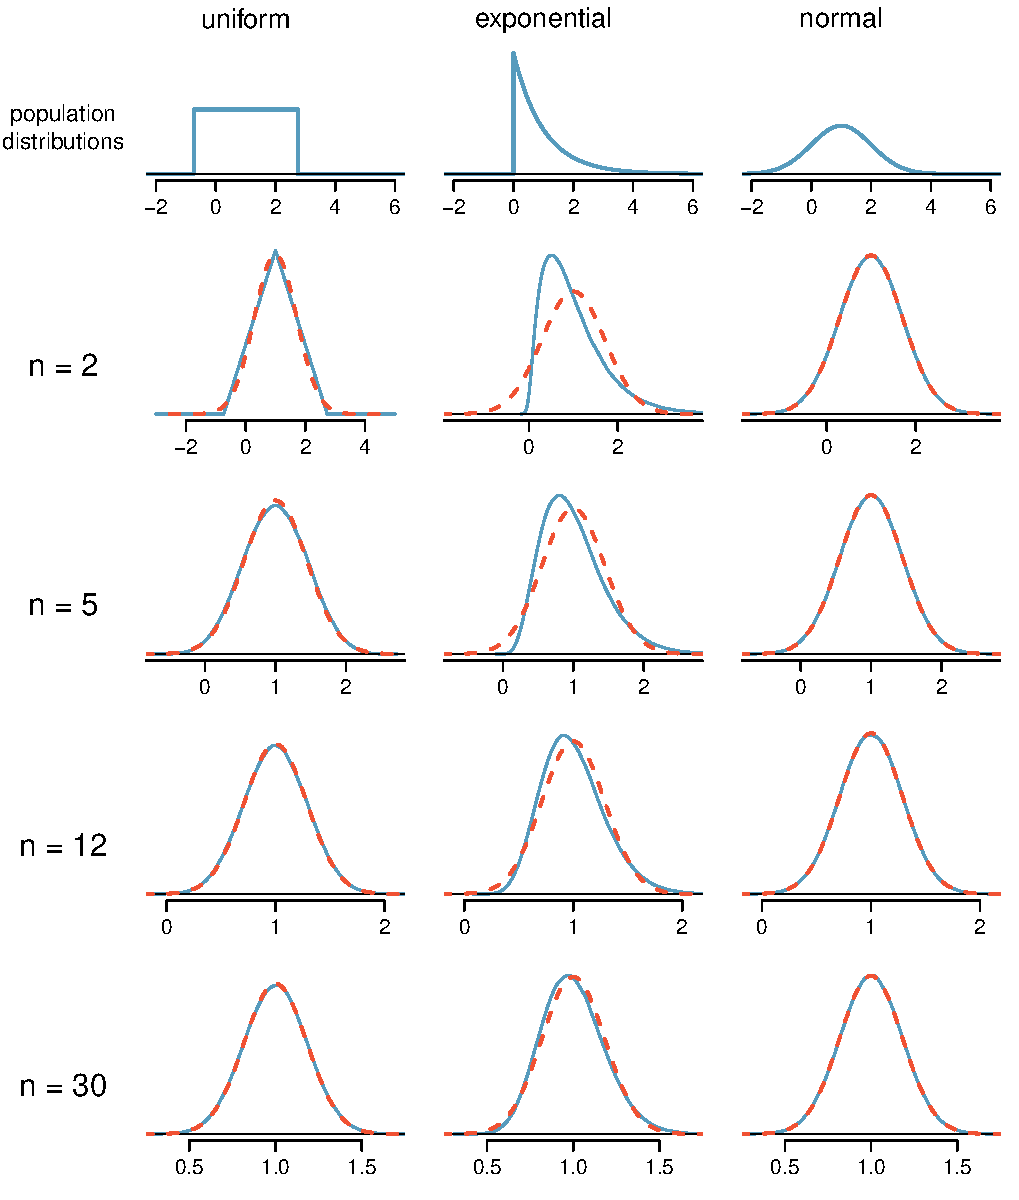
\includegraphics[width=\textwidth]{ch_distributions/figures/cltSimulations/cltSimulations}
   \caption{Sampling distributions for the mean at different sample sizes and for three different distributions. The dashed red lines show normal distributions.}
   \label{cltSimulations}
\end{figure}

The left panel in the $n=2$ row represents the sampling distribution of $\bar{x}$ if it is the sample mean of two observations from the uniform distribution shown. The dashed line represents the closest approximation of the normal distribution. Similarly, the center and right panels of the $n=2$ row represent the respective distributions of $\bar{x}$ for data from exponential and log-normal distributions.

\begin{exercisewrap}
\begin{nexercise}
Examine the distributions in each row of Figure~\ref{cltSimulations}. What do you notice about the sampling distribution of the mean as the sample size, $n$, becomes larger?\footnotemark
\end{nexercise}
\end{exercisewrap}
\footnotetext{The normal approximation becomes better as larger samples are used. However, in the case when the population is normally distributed, the normal distribution of the sample mean is normal for all sample sizes.}

\begin{examplewrap}
\begin{nexample}{In general, would normal approximation for a sample mean be appropriate when the sample size is at least 30?}
Yes, the sampling distributions when $n = 30$ all look very much like the normal distribution.

However, the more non-normal a population distribution, the larger a sample size is necessary for the sampling distribution to look nearly normal.
\end{nexample}
\end{examplewrap}

\begin{onebox}{Determining if the sample mean is normally distributed}
If the population is normal, the sampling distribution of $\bar{x}$ will be normal for any sample size. \\[2mm]
The less normal the population, the larger $n$ needs to be for the sampling distribution of $\bar{x}$ to be nearly normal. However, a good rule of thumb is that for almost all populations, the sampling distribution of $\bar{x}$ will be approximately normal if $n \ge 30$.\end{onebox}

This brings us to the \term{Central Limit Theorem}, the most fundamental theorem in Statistics.

\begin{onebox}{Central Limit Theorem}
When taking a random sample of independent observations from a population with a fixed mean and standard deviation, the distribution of $\bar{x}$ approaches the normal distribution as $n$ increases.\end{onebox}

\D{\newpage}

\begin{examplewrap}
\begin{nexample}{Sometimes we do not know what the population distribution looks like. We have to infer it based on the distribution of a single sample. Figure~\ref{pokerProfitsCanApplyNormalToSampMean} shows a histogram of 20 observations. These represent winnings and losses from 20 consecutive days of a professional poker player. Based on this sample data, can the normal approximation be applied to the distribution of the sample mean?}
We should consider each of the required conditions.
\begin{itemize}
\setlength{\itemsep}{0mm}
\item[(1)] These are referred to as \term{time series data}, because the data arrived in a particular sequence. If the player wins on one day, it may influence how she plays the next. To make the assumption of independence we should perform careful checks on such data.
\item[(2)] The sample size is 20, which is smaller than 30.
\item[(3)] There are two outliers in the data, both quite extreme, which suggests the population may not be normal and instead may be very strongly skewed or have distant outliers. Outliers can play an important role and affect the distribution of the sample mean and the estimate of the standard deviation of the sample mean.
\end{itemize}
Since we should be skeptical of the independence of observations and the extreme upper outliers pose a challenge, we should not use the normal model for the sample mean of these 20 observations. If we can obtain a much larger sample, then the concerns about skew and outliers would no longer apply.
\end{nexample}
\end{examplewrap}

\begin{figure}[ht]
   \centering
   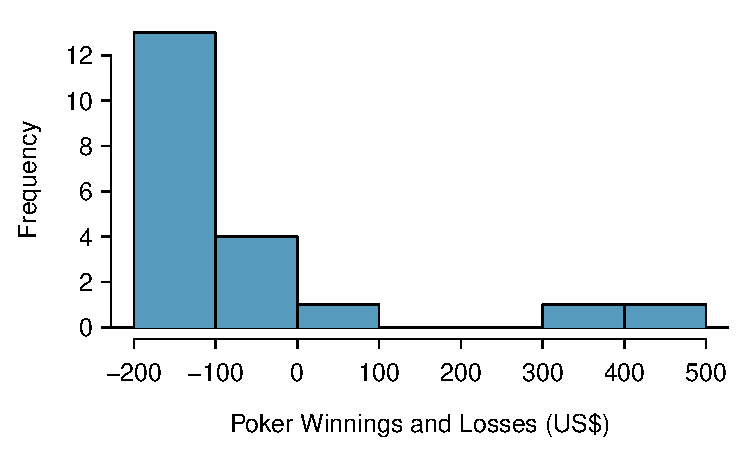
\includegraphics[height=58mm]{ch_distributions/figures/pokerProfitsCanApplyNormalToSampMean/pokerProfitsCanApplyNormalToSampMean}
   \caption{Sample distribution of poker winnings. These data include two very clear outliers. These are problematic when considering the normality of the sample mean. For example, outliers are often an indicator of very strong skew\index{skew!example: very strong}.}
   \label{pokerProfitsCanApplyNormalToSampMean}
\end{figure}

\begin{onebox}{Examine data structure when considering independence}
{Some data sets are collected in such a way that they have a natural underlying structure between observations, e.g. when observations occur consecutively. Be especially cautious about independence assumptions regarding such data sets.}
\end{onebox}

\begin{onebox}{Watch out for strong skew and outliers}
{Strong skew in the population is often identified by the presence of clear outliers in the data. If a data set has prominent outliers, then a larger sample size will be needed for the sampling distribution of $\bar{x}$ to be normal. There are no simple guidelines for what sample size is big enough for each situation. However, we can use the rule of thumb that, in general, an $n$ of at least 30 is sufficient for most cases.}
\index{skew!strongly skewed guideline}
\end{onebox}
\index{Central Limit Theorem|)}


\D{\newpage}

%%
\subsection[Normal approximation for the sampling distribution of $\bar{x}$]{Normal approximation for the sampling distribution of \pmb{$\bar{x}$}}

At the beginning of this chapter, we used normal approximation for populations or for data that had an approximately normal distribution. When appropriate conditions are met, we can also use the normal approximation to estimate probabilities about a sample average. We must remember to verify that the conditions are met and use the mean $\mu_{\bar{x}}$ and standard deviation $\sigma_{\bar{x}}$ for the sampling distribution of the sample average.

\begin{onebox}{Three important facts about the distribution of a sample mean \pmb{\MakeLowercase{$\bar{x}$}}}
Consider taking a simple random sample from a large population.
\begin{enumerate}
\setlength{\itemsep}{0mm}
\item The mean of a sample mean is denoted by $\mu_{\bar{x}}$, and it is equal to $\mu$.
\item The SD of a sample mean is denoted by $\sigma_{\bar{x}}$, and it is equal to $\frac{\sigma}{\sqrt{n}}$.
\item When the population is normal or when $n\ge 30$, the sample mean closely follows a normal distribution. 
\end{enumerate}\end{onebox}

\begin{examplewrap}
\begin{nexample}{
In the 2012 Cherry Blossom 10 mile run, the average time for all of the runners is 94.52 minutes with a standard deviation of 8.97 minutes. The distribution of run times is approximately normal. Find the probabiliy that a randomly selected runner completes the run in less than 90 minutes.}Because the distribution of run times is approximately normal, we can use normal approximation.
\begin{align*}
&Z = \frac{x - \mu}{\sigma}=\frac{90-94.52}{8.97}=-0.504 \\
&P(Z < -0.504) = 0.3072
\end{align*}
There is a 30.72\% probability that a randomly selected runner will complete the run in less than 90~minutes.
\end{nexample}
\end{examplewrap}

\begin{examplewrap}
\begin{nexample}{
Find the probabiliy that the average of 20 runners is less than 90~minutes.}
Here, $n=20<30$, but the distribution of the population, that~is, the distribution of run times is stated to be approximately normal. Because of this, the sampling distribution will be normal for any sample size.
\begin{align*}
&\sigma_{\bar{x}}=\frac{\sigma}{\sqrt{n}}=\frac{8.97}{\sqrt{20}}=2.01 \\
&Z = \frac{\bar{x} - \mu_{\bar{x}}}{\sigma_{\bar{x}}}=\frac{90-94.52}{2.01}=-2.25\\
&P(Z < -2.25) = 0.0123
\end{align*}
There is a 1.23\% probability that the average run time of 20 randomly selected runners will be less than 90~minutes.
\end{nexample}
\end{examplewrap}

\D{\newpage}

\begin{examplewrap}
\begin{nexample}{
The average of all the runners' ages is 35.05 years with a standard deviation of $\sigma = 8.97$. The distribution of age is somewhat skewed. What is the probability that a randomly selected runner is older than 37 years?}Because the distribution of age is skewed and is not normal, we cannot use normal approximation for this problem. In order to answer this question, we would need to look at all of the data.
\end{nexample}
\end{examplewrap}

\begin{exercisewrap}
\begin{nexercise}
What is the probability that the average of 50 randomly selected runners is greater than 37 years?\footnotemark
\end{nexercise}
\end{exercisewrap}
\footnotetext{Because $n=50\ge 30$, the sampling distribution of the mean is approximately normal, so we can use normal approximation for this problem. The mean is given as 35.05 years.
\begin{align*}
&\sigma_{\bar{x}}
	= \frac{\sigma}{\sqrt{n}}
	= \frac{8.97}{\sqrt{50}}=1.27
&&z=\frac{\bar{x}-\mu_{\bar{x}}}{\sigma_{\bar{x}}} = \frac{37-35.05}{1.27}=1.535
&&P(Z > 1.535) = 0.062
\end{align*}
There is a 6.2\% chance that the average age of 50 runners will be greater than 37.} 

\begin{onebox}{Remember to divide by $\pmb{\sqrt{\MakeLowercase{n}}}$}
When finding the probability that an \emph{average} or mean is greater or less than a particular value, remember to divide the standard deviation of the population by $\sqrt{n}$ to calculate the correct~SD.\end{onebox}


\D{\newpage}

%%
\subsection*{Section summary}

\begin{itemize}
\item The symbol $\bar{x}$ denotes the sample average.  $\bar{x}$ for any particular sample is a number.  However, $\bar{x}$ can vary from sample to sample.  The distribution of all possible values of $\bar{x}$ for repeated samples of a fixed size from a certain population is called the \term{sampling distribution} of $\bar{x}$.

\item The standard deviation of $\bar{x}$ describes the typical error or distance of the sample mean from the population mean.  It also tells us how much the sample mean is likely to vary from one random sample to another.  

\item The standard deviation of $\bar{x}$ will be \textit{smaller} than the standard deviation of the population by a factor of $\sqrt{n}$.  The larger the sample, the better the estimate tends to be.

\item Consider taking a simple random sample from a population with a fixed mean and standard deviation.  The \term{Central Limit Theorem} ensures that regardless of the shape of the original population, as the sample size increases, the distribution of the sample average $\bar{x}$ becomes more normal.  

\item Three important facts about the sampling distribution of the sample average $\bar{x}$:
\begin{itemize}\vspace{-1mm}
\setlength{\itemsep}{0mm}
\item The mean of a sample mean is denoted by $\mu_{\bar{x}}$, and it is equal to $\mu$. (\textit{center})
\item The SD of a sample mean is denoted by $\sigma_{\bar{x}}$, and it is equal to $\frac{\sigma}{\sqrt{n}}$.  (\textit{spread})
\item When the population is normal or when $n\ge 30$, the sample mean closely follows a normal distribution.   (\textit{shape})
\end{itemize}

\item These facts are used when solving the following two types of \textbf{normal approximation} problems involving a \emph{sample mean} or a \emph{sample sum}.  
\begin{itemize}
\item[A:] \textit{Find the probability that a sample average will be greater/less than a certain value}.
\begin{enumerate}\vspace{-1mm}
\setlength{\itemsep}{0mm}
\item Verify that the population is approximately normal or that $n \ge 30$.
\item Calculate the Z-score.  Use $\mu_{\bar{x}}=\mu$ and $\sigma_{\bar{x}}=\frac{\sigma}{\sqrt{n}}$ to standardize the sample average.  
\item Find the appropriate area under the normal curve.  
\end{enumerate}

\item[B:] \textit{Find the probability that a sample sum/total will be greater/less than a certain value}.
\begin{enumerate}\vspace{-1mm}
\setlength{\itemsep}{0mm}
\item Convert the sample sum into a sample average, using $\bar{x} = \frac{sum}{n}$.  
\item Do steps 1-3 from Part A above.
\end{enumerate}
\end{itemize}
\end{itemize}


%%%%%%%%%%Section exercises
{\exercisesheader{}

% 7 - ages_pennies_1

\eoce{\qt{Ages of pennies, Part I \label{ages_pennies_1}} The histogram below shows the distribution of ages of pennies at a bank. 

\noindent\begin{minipage}[c]{0.54\textwidth}
\begin{parts}
\item Describe the distribution.
\item Sampling distributions for means from simple random samples of 5, 30, and 100 pennies is shown in the histograms below. Describe the shapes of these distributions and comment on whether they look like what you would expect to see based on the Central Limit Theorem.
\end{parts}
\end{minipage}
\begin{minipage}[c]{0.44\textwidth}
\begin{center}
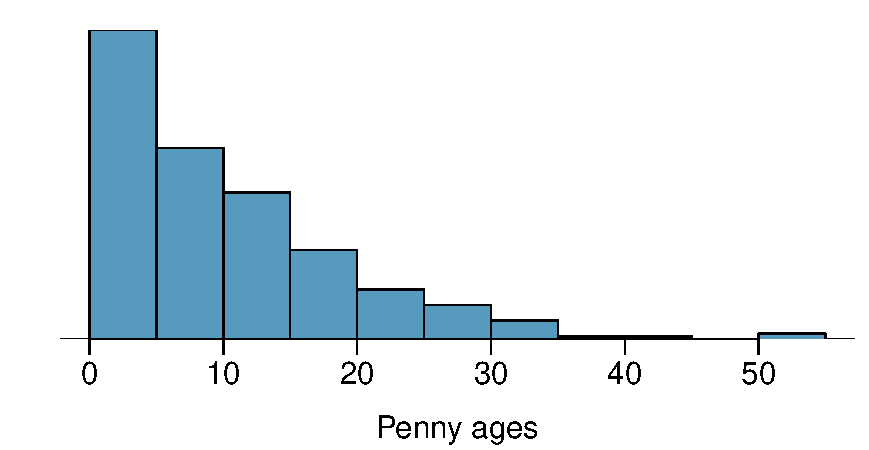
\includegraphics[width=\textwidth]{ch_distributions/figures/eoce/ages_pennies_1/penniesAges_pop} 
\end{center}
\end{minipage}\vspace{-1mm}
\begin{center}
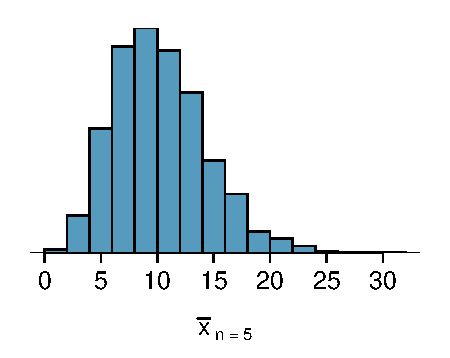
\includegraphics[width=0.325\textwidth]{ch_distributions/figures/eoce/ages_pennies_1/penniesAges_n5} 
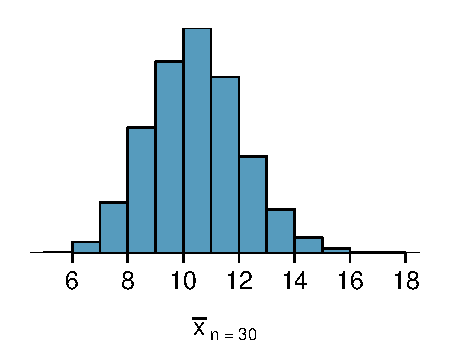
\includegraphics[width= 0.325\textwidth]{ch_distributions/figures/eoce/ages_pennies_1/penniesAges_n30} 
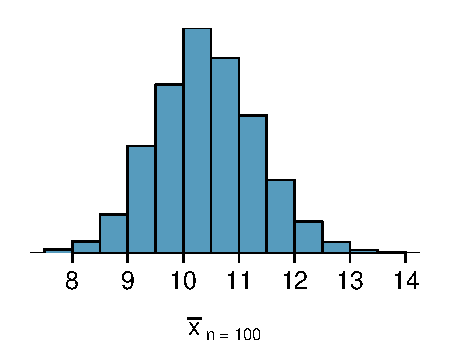
\includegraphics[width= 0.325\textwidth]{ch_distributions/figures/eoce/ages_pennies_1/penniesAges_n100} 
\end{center}
}{}

% 8 - ages_pennies_2

\eoce{\qt{Ages of pennies, Part II\label{ages_pennies_2}} The mean age of the pennies from Exercise~\ref{ages_pennies_1} is 10.44 years with a standard deviation of 9.2 years. Using the Central Limit Theorem, calculate the means and standard deviations of the distribution of the mean from random samples of size 5, 30, and 100. Comment on whether the sampling distributions shown in Exercise~\ref{ages_pennies_1} agree with the values you compute.
}{}

% 9 - housing_prices

\eoce{\qt{Housing prices\label{housing_prices}} \videosolution{ahss_eoce_sol-housing_prices} A housing survey was conducted to 
determine the price of a typical home in Topanga, CA. The mean price of a house 
was roughly \$1.3 million with a standard deviation of \$300,000. There were no 
houses listed below \$600,000 but a few houses above \$3 million.
\begin{parts}
\item Is the distribution of housing prices in Topanga symmetric, right skewed, 
or left skewed? \textit{Hint:} Sketch the distribution.
\item Would you expect most houses in Topanga to cost more or less than \$1.3 
million?
\item Can we estimate the probability that a randomly chosen house in Topanga 
costs more than \$1.4 million using the normal distribution?
\item What is the probability that the mean of 60 randomly chosen houses in 
Topanga is more than \$1.4 million?
\item How would doubling the sample size affect the standard deviation of the 
mean?
\end{parts}
}{}

% 10 - stats_final_scores

\eoce{\qt{Stats final scores\label{stats_final_scores}} Each year about 1500 students 
take the introductory statistics course at a large university. This year scores 
on the final exam are distributed with a median of 74 points, a mean of 70 
points, and a standard deviation of 10 points. There are no students who scored 
above 100 (the maximum score attainable on the final) but a few students scored 
below 20 points.
\begin{parts}
\item Is the distribution of scores on this final exam symmetric, right skewed, 
or left skewed?
\item Would you expect most students to have scored above or below 70 points?
\item Can we calculate the probability that a randomly chosen student scored 
above 75 using the normal distribution?
\item What is the probability that the average score for a random sample of 40 
students is above 75?
\item How would cutting the sample size in half affect the standard deviation of 
the mean?
\end{parts}
}{}

% 11 - identify_dist_symm_pop

\eoce{\qt{Identify distributions, Part I\label{identify_dist_symm_pop}} Four plots 
are presented below. The plot at the top is a distribution for a population. The 
mean is 10 and the standard deviation is 3. Also shown below is a distribution 
of (1) a single random sample of 100 values from this population, (2) a 
distribution of 100 sample means from random samples with size 5, and (3) a 
distribution of 100 sample means from random samples with size 25. Determine 
which plot (A, B, or C) is which and explain your reasoning.
\begin{center}
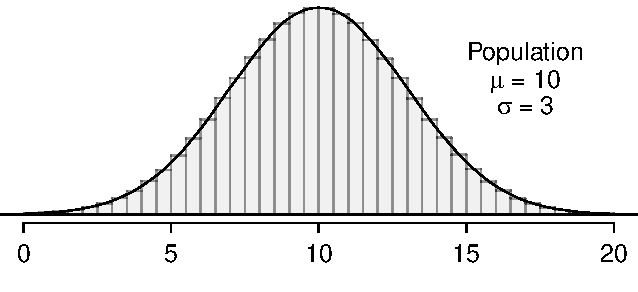
\includegraphics[width=0.55\textwidth]{ch_distributions/figures/eoce/identify_dist_symm_pop/identify_dist_symm_pop.pdf} \\
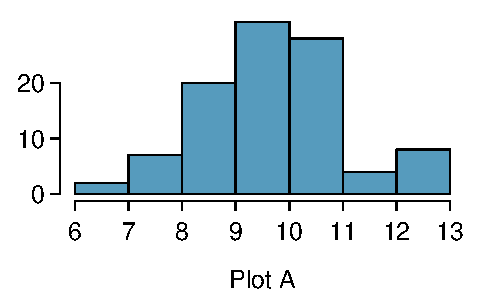
\includegraphics[width=0.325\textwidth]{ch_distributions/figures/eoce/identify_dist_symm_pop/identify_dist_symm_sampling_n5.pdf}
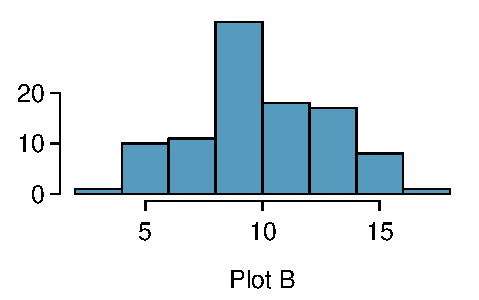
\includegraphics[width=0.325\textwidth]{ch_distributions/figures/eoce/identify_dist_symm_pop/identify_dist_symm_samp.pdf}
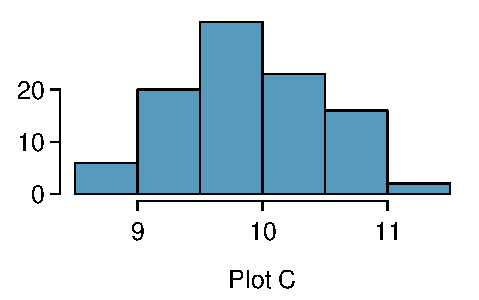
\includegraphics[width=0.325\textwidth]{ch_distributions/figures/eoce/identify_dist_symm_pop/identify_dist_symm_sampling_n25.pdf}
\end{center}
}{}

% 12 - identify_dist_ls_pop

\eoce{\qt{Identify distributions, Part II\label{identify_dist_ls_pop}} Four plots are presented below. The plot at 
the top is a distribution for a population. The mean is 60 and the standard 
deviation is 18. Also shown below is a distribution of (1) a single random 
sample of 500 values from this population, (2) a distribution of 500 sample 
means from random samples of each size 18, and (3) a distribution of 500 sample 
means from random samples of each size 81. Determine which plot (A, B, or C) is 
which and explain your reasoning.
\begin{center}
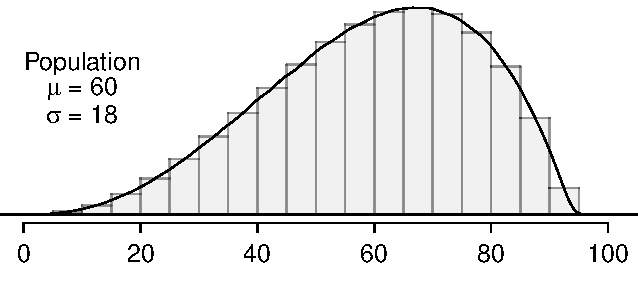
\includegraphics[width=0.55\textwidth]{ch_distributions/figures/eoce/identify_dist_ls_pop/identify_dist_ls_pop.pdf}
\end{center}
\begin{center}
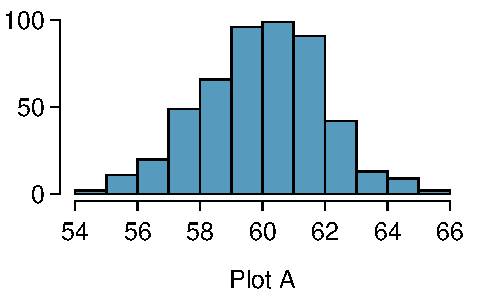
\includegraphics[width=0.325\textwidth]{ch_distributions/figures/eoce/identify_dist_ls_pop/identify_dist_ls_sampling_n81.pdf}
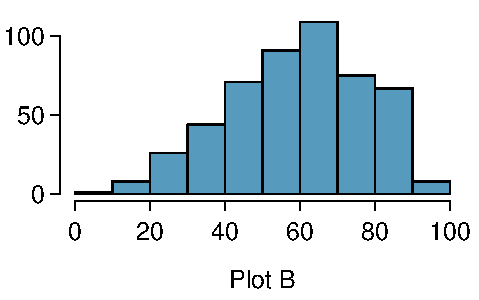
\includegraphics[width=0.325\textwidth]{ch_distributions/figures/eoce/identify_dist_ls_pop/identify_dist_ls_samp.pdf}
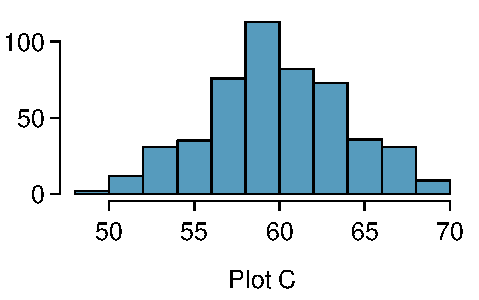
\includegraphics[width=0.325\textwidth]{ch_distributions/figures/eoce/identify_dist_ls_pop/identify_dist_ls_sampling_n18.pdf}
\end{center}
}{}

% 13 - penny_weights

\eoce{\qt{Weights of pennies\label{penny_weights}} The distribution of weights of 
United States pennies is approximately normal with a mean of 2.5 grams and a 
standard deviation of 0.03 grams.
\begin{parts}
\item What is the probability that a randomly chosen penny weighs less than 2.4 
grams?
\item Describe the sampling distribution of the mean weight of 10 randomly 
chosen pennies.
\item What is the probability that the mean weight of 10 pennies is less than 
2.4 grams?
\item Sketch the two distributions (population and sampling) on the same scale.
\item Could you estimate the probabilities from (a) and (c) if the weights of pennies had a skewed distribution?
\end{parts}
}{}

% 14 - cflbs

\eoce{\qt{CFLBs\label{cflbs}} A manufacturer of compact fluorescent light bulbs advertises 
that the distribution of the lifespans of these light bulbs is nearly normal with 
a mean of 9,000 hours and a standard deviation of 1,000 hours.
\begin{parts}
\item What is the probability that a randomly chosen light bulb lasts more than 
10,500 hours?
\item Describe the distribution of the mean lifespan of 15 light bulbs. 
\item What is the probability that the mean lifespan of 15 randomly chosen light 
bulbs is more than 10,500 hours?
\item Sketch the two distributions (population and sampling) on the same scale.
\item Could you estimate the probabilities from parts~(a) and~(c) if the 
lifespans of light bulbs had a skewed distribution?
\end{parts}
}{}

% 15 - songs_on_ipod

\eoce{\qt{Songs on an iPod\label{songs_on_ipod}} Suppose an iPod has 3,000 songs. The 
histogram below shows the distribution of the lengths of these songs. We also 
know that, for this iPod, the mean length is 3.45 minutes and the standard 
deviation is 1.63 minutes.
\begin{center}
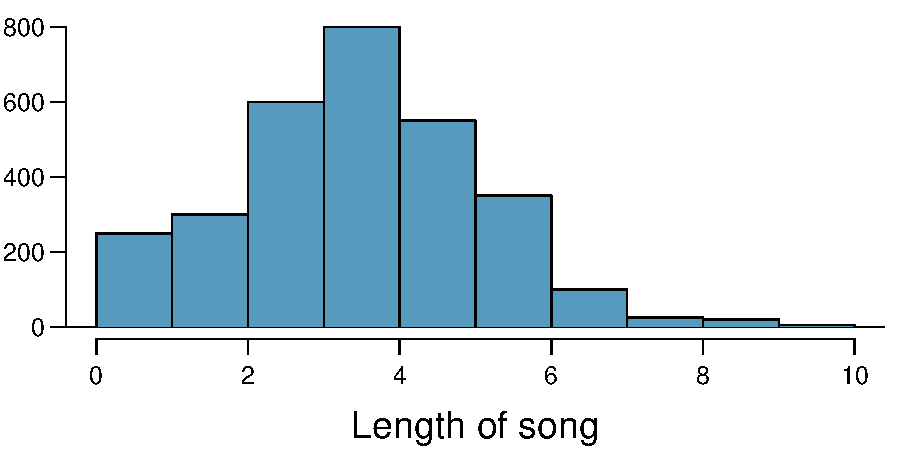
\includegraphics[width=0.5\textwidth]{ch_distributions/figures/eoce/songs_on_ipod/songs_on_ipod_pop_hist.pdf}
\end{center}
\begin{parts}
\item Calculate the probability that a randomly selected song lasts more than 5 
minutes.
\item You are about to go for an hour run and you make a random playlist of 15 songs. What is the probability that your playlist lasts for the entire duration 
of your run? \textit{Hint:} If you want the playlist to last 60 minutes, what should be the minimum average length of a song?
\item You are about to take a trip to visit your parents and the drive is 6 hours. You make a random playlist of 100 songs. What is the probability that your playlist lasts the entire drive?
\end{parts}
}{}

% 16 - spray_paint_2

\eoce{\qt{Spray paint, Part II\label{spray_paint_2}} Suppose the area that can be painted using a 
single can of spray paint is slightly variable and follows a nearly normal 
distribution with a mean of 25 square feet and a standard deviation of 3 square 
feet. 
\begin{parts}
\item What is the probability that the area covered by a can of spray paint is 
more than 27 square feet?
\item Suppose you want to spray paint an area of 540 square feet using 20 cans 
of spray paint. On average, how many square feet must each can be able to cover 
to spray paint all 540 square feet?
\item What is the probability that you can cover a 540 square feet area using 20 
cans of spray paint?
\item If the area covered by a can of spray paint had a slightly skewed 
distribution, could you still calculate the probabilities in parts~(a) and~(c) 
using the normal distribution?
\end{parts}
}{}

% 17 - wireless_routers

\eoce{\qt{Wireless routers\label{wireless_routers}} John is shopping for wireless routers and is overwhelmed by the number of available options. In order to get a feel for the average price, he takes a random sample of 75 routers and finds that the average price for this sample is \$75 and the standard deviation is \$25. 
\begin{parts}
\item Based on this information, how much variability should he expect to see in the mean prices of repeated samples, each containing 75 randomly selected wireless routers?
\item A consumer website claims that the average price of routers is \$80. Is a true average of \$80 consistent with John's sample?
\end{parts}
}{}

% 18 - betting_on_dinner_2

\eoce{\qt{Betting on dinner, Part II\label{betting_on_dinner_2}} Exercise~\ref{betting_on_dinner_1} introduces a promotion at a restaurant where prices of menu items are determined randomly following some underlying distribution. We are told that the price of basket of fries is drawn from a normal distribution with mean 6 and standard deviation of 2. You want to get 5 baskets of fries but you only have \$28 in your pocket. What is the probability that you would have enough money to pay for all five baskets of fries?
}{}
}


%__________________________________________
\section{Geometric distribution}
\label{geomDist}

\sectionintro{
\noindent%
How many times should we expect to roll a die until we get a \resp{1}?
How many people should we expect to see at a hospital until we get someone with blood type O+?
These questions can be answered using the geometric distribution.
We will see that unlike with the distribution of a sample mean, the shape of the geometric distribution is never normal.

%%
\subsection*{Learning objectives}

\begin{enumerate}
\setlength{\itemsep}{0mm}

\item Determine if a scenario is geometric.

\item Calculate the probabilities of the possible values of a geometric random variable.

\item Find and interpret the mean (expected value) of a geometric distribution.

\item Understand the shape of the geometric distribution.

\end{enumerate}
}

%%
\subsection{Bernoulli distribution}
\label{bernoulli}

%\newcommand{\insureSprob}{0.7}
%\newcommand{\insureSperc}{70\%}
%\newcommand{\insureFprob}{0.3}
%\newcommand{\insureFperc}{30\%}
%\newcommand{\insureDistA}{0.7}
%\newcommand{\insureDistB}{0.21}
%\newcommand{\insureDistC}{0.063}
%\newcommand{\insureDistD}{0.019}
%\newcommand{\insureDistE}{0.006}
%\newcommand{\insureCDistA}{0.7}
%\newcommand{\insureCDistB}{0.91}
%\newcommand{\insureCDistC}{0.973}
%\newcommand{\insureCDistCComplement}{0.027}
%\newcommand{\insureCDistD}{0.992}
%\newcommand{\insureCDistE}{0.998}
%\newcommand{\insureGeomMean}{1.43}

\index{distribution!Bernoulli|(}

We begin by revisiting a scenario encountered when studying the binomial formula (section~\ref{binomialForm}), and we formalize the notion of a yes/no variable.

Many health insurance plans in the United States have
a deductible, where the insured individual is responsible
for costs up to the deductible, and then the costs above
the deductible are shared between the individual and
insurance company for the remainder of the year.

Suppose a health insurance company found that \insureSperc{} of the
people they insure stay below their deductible in any given year.
Each of these people can be thought of as a \term{trial}.
We label a person a \term{success} if her healthcare costs
do not exceed the deductible.
We label a person a \term{failure} if she does exceed her
deductible in the year.
Because \insureSperc{} of the individuals will not exceed their deductible,
we denote the \term{probability of a success} as
$p = \insureSprob{}$.
The probability of a failure is sometimes denoted with
$q = 1 - p$, which would be \insureFprob{} in for the insurance
example.

When an individual trial only has two possible outcomes, often
labeled as \resp{success} or \resp{failure}, it is called a
\termsub{Bernoulli random variable}{distribution!Bernoulli}.
We chose to label a person who does not exceed her deductible
as a ``success'' and all others as ``failures''.
However, we could just as easily have reversed these labels.
The mathematical framework we will build does not depend
on which outcome is labeled a success and which a failure,
as long as we are consistent.

\D{\newpage}

Bernoulli random variables are often denoted as \resp{1}
for a success and \resp{0} for a failure.
In addition to being convenient in entering data,
it is also mathematically handy.
Suppose we observe ten trials:
\begin{center}
\resp{1} \resp{1} \resp{1} \resp{0} \resp{1} \resp{0} \resp{0} \resp{1} \resp{1} \resp{0}
\end{center}
Then the \term{sample proportion}, $\hat{p}$, is the
sample mean of these observations:
\begin{align*}
\hat{p} = \frac{\text{\# of successes}}{\text{\# of trials}}
    = \frac{1+1+1+0+1+0+0+1+1+0}{10} = 0.6
\end{align*}%
This mathematical inquiry of Bernoulli random variables can
be extended even further.
%\Comment{Maybe the next footnote should instead be an EOCE?}
Because \resp{0} and \resp{1} are numerical outcomes,
we can define the {mean} and {standard deviation}
of a Bernoulli random variable.\footnote{If ${p}$ is the true probability of a success, then the mean of a Bernoulli random variable $X$ is given by
\begin{align*}
\mu = E(X) &=  0\cdot P(X = 0) +  1\cdot P(X=1) \\
	&=   0\cdot (1 - p) +  1\cdot p = 0 + p = p
\end{align*}
Similarly, the variance of $X$ can be computed:
\begin{align*}
\sigma^2 &= {(0-p)^2\cdot P(X=0) + (1-p)^2\cdot P(X=1)} \\
	&= {p^2\cdot (1-p) + (1-p)^2\cdot p} = {p(1-p)}
\end{align*}
The standard deviation is $\sigma=\sqrt{p(1-p)}$.}

\begin{onebox}{Bernoulli random variable}
%  A Bernoulli random variable has exactly two possible
%  outcomes, often labeled \resp{1} for the ``success''
%  outcome and \resp{0} for the ``failure'' outcome.\vspace{3mm}
  If $X$ is a random variable that takes value 1 with
  probability of success $p$ and 0 with probability $1-p$,
  then $X$ is a Bernoulli random variable with mean
  and standard deviation
  \begin{align*}
  \mu &= p
      &\sigma&= \sqrt{p(1-p)}
  \end{align*}
\end{onebox}

In general, it is useful to think about a Bernoulli random variable as a random process with only two outcomes: a success or failure. Then we build our mathematical framework using the numerical labels \resp{1} and \resp{0} for successes and failures, respectively.

\index{distribution!Bernoulli|)}



%%
\subsection{Geometric distribution}

\index{distribution!geometric|(}

The \termsub{geometric distribution}{distribution!geometric}
is used to describe how
many trials it takes to observe a success.
Let's first look at an example.

\begin{examplewrap}
\begin{nexample}{Suppose we are working at the insurance
    company and need to find a case where the person did
    not exceed her (or his) deductible as a case study.
    If the probability a person will not exceed her
    deductible is \insureSprob{} and we are drawing people
    at random, what are the chances that the first person
    will not have exceeded her deductible, i.e. be a success?
    The second person?
    The third?
    What about the probability that we pull $x - 1$ cases before we find
    the first success, i.e. the first success is the
    $x^{th}$ person?
    (If the first success is the fifth person, then we say $x=5$.)}
  \label{waitForDeductible}%
  The probability of stopping after the first person is just
  the chance the first person will not exceed her (or his)
  deductible:~\insureSprob{}.
The probability the second person is the first to exceed
  her deductible is  \begin{align*}
  &P(\text{second person is the first to exceed deductible})  \\
  &\quad
    = P(\text{the first won't, the second will})
    = (\insureFprob{})(\insureSprob{})
    = \insureDistB{}
  \end{align*}
  Likewise, the probability it will be the third case is
  $(\insureFprob{})(\insureFprob{})(\insureSprob{})
    = \insureDistC$.

  If the first success is on the $x^{th}$ person,
  then there are $x-1$ failures and finally 1 success,
  which corresponds to the probability
  $(\insureFprob{})^{x-1}(\insureSprob{})$.
  This is the same as
  $(1-\insureSprob{})^{x-1}(\insureSprob{})$.
\end{nexample}
\end{examplewrap}

\D{\newpage}

Example~\ref{waitForDeductible} illustrates what the
\termsub{geometric distribution}{distribution!geometric},
which describes the waiting
time until a success for
\term{independent and identically distributed (iid)}
Bernoulli random variables.
In this case, the \emph{independence} aspect just means
the individuals in the example don't affect each other,
and \emph{identical} means they each have the same probability
of success.

The geometric distribution from Example~\ref{waitForDeductible} is shown in Figure~\ref{geometricDist70}. In general, the probabilities for a geometric distribution decrease \term{exponentially} fast.

\begin{figure}[h]
  \centering
  \Figure{0.75}{geometricDist70}
  \caption{The geometric distribution when the probability
      of success is $p = \insureSprob{}$.}
  \label{geometricDist70}
\end{figure}

While this text will not derive the formulas for the mean (expected) number of trials needed to find the first success or the standard deviation or variance of this distribution, we present general formulas for each.

\begin{onebox}{Geometric Distribution}
  \index{distribution!geometric|textbf}%
  Let X have a geometric distribution with one parameter $p$, where $p$ is the probability of a success in one trial.   Then the
  probability of finding the first success in the
  $x^{th}$ trial is given by\vspace{-1.5mm}
  \begin{align*}
  P(X = x) = (1-p)^{x-1}p
  \end{align*}
where $x=1,2,3,\dots$\\
\\
  The mean (i.e. expected value) and standard deviation of this wait time are given by
  \begin{align*}
  \mu_{\scriptscriptstyle{X}} = \frac{1}{p}
      \qquad \sigma_{\scriptscriptstyle{X}} = \frac{\sqrt{1-p\ }}{p}
  \end{align*}
\end{onebox}

It is no accident that we use the symbol $\mu$ for both the mean and expected value. The mean and the expected value are one and the same.

It takes, on average, $1/p$ trials to get a success under the geometric distribution. This mathematical result is consistent with what we would expect intuitively. If the probability of a success is high (e.g. 0.8), then we don't usually wait very long for a success: $1/0.8 = 1.25$ trials on average. If the probability of a success is low (e.g. 0.1), then we would expect to view many trials before we see a success: $1/0.1 = 10$ trials.

\D{\newpage}

\begin{exercisewrap}
\begin{nexercise}
The probability that a particular case would not exceed their
deductible is said to be \insureSprob{}.
If we were to examine cases until we found one that where
the person did not exceed her deductible, how many cases should
we expect to check?\footnotemark{}
\end{nexercise}
\end{exercisewrap}
\footnotetext{We would expect to see about
    $1 / \insureSprob{} \approx \insureGeomMean{}$
    individuals to find the first success.}

\begin{examplewrap}
\begin{nexample}{What is the chance that we would find
    the first success within the first 3 cases?}
  \label{insureFirstSuccessInLT4}%
  This is the chance the first ($X=1$), second ($X=2$),
  or third ($X=3$) case is the first success, which are three
  disjoint outcomes.
  Because the individuals in the sample are randomly sampled
  from a large population, they are independent.
  We compute the probability of each case and add the separate
  results:
  \begin{align*}
  &P(X=1, 2, \text{ or }3) \\
    & \quad = P(X=1)+P(X=2)+P(X=3) \\
    & \quad = (\insureFprob{})^{1-1}(\insureSprob{})
        + (\insureFprob{})^{2-1}(\insureSprob{})
        + (\insureFprob{})^{3-1}(\insureSprob{}) \\
    & \quad = \insureCDistC{}
  \end{align*}
  There is a probability of \insureCDistC{} that we would
  find a successful case within 3 cases.
\end{nexample}
\end{examplewrap}

\begin{exercisewrap}
\begin{nexercise}
Determine a more clever way to solve Example~\ref{insureFirstSuccessInLT4}.
Show that you get the same result.\footnotemark{}
\end{nexercise}
\end{exercisewrap}
\footnotetext{First find the probability of the complement:
  $P($no success in first 3~trials$)
      = \insureFprob{}^3 = \insureCDistCComplement{}$.
  Next, compute one minus this probability:
  $1 - P($no success in 3 trials$)
      = 1 - \insureCDistCComplement{}
      = \insureCDistC{}$.}

\begin{examplewrap}
\begin{nexample}{Suppose a car insurer has determined
    that 88\% of its drivers will not exceed their deductible
    in a given year.
    If someone at the company were to randomly draw
    driver files until they found one that had not exceeded
    their deductible, what is the expected number of drivers
    the insurance employee must check?
    What is the standard deviation of the number of driver files
    that must be drawn?}
  \label{carInsure08DrawOne}%
  In this example, a success is again when someone will not
  exceed the insurance deductible, which has probability
  $p = 0.88$.
  The expected number of people to be checked is
  $1 / p = 1 / 0.88 = 1.14$ and the standard deviation is
  $\frac{\sqrt{1-p\ }}{p}=\frac{\sqrt{1-0.88\ }}{0.88} = 0.39$.
\end{nexample}
\end{examplewrap}

\begin{exercisewrap}
\begin{nexercise}
Using the results from Example~\ref{carInsure08DrawOne},
$\mu_{\scriptscriptstyle{X}} = 1.14$ and $\sigma_{\scriptscriptstyle{X}} = 0.39$, would it be appropriate
to use the normal model to find what proportion
of experiments would end in 3 or fewer trials?\footnotemark{}
\end{nexercise}
\end{exercisewrap}
\footnotetext{No. The geometric distribution is always
  right skewed and can never be well-approximated by the
  normal model.}

The independence assumption is crucial to the geometric
distribution's accurate description of a scenario.
Mathematically, we can see that to construct the probability
of the success on the $x^{th}$ trial, we had to use the
General Multiplication Rule for independent processes.
It is no simple task to generalize the geometric model
for dependent trials.

\index{distribution!geometric|)}


\D{\newpage}

%%
\subsection*{Section summary}

\begin{itemize}
\item It is useful to model yes/no, success/failure with the values 1 and 0, respectively. We call the \term{probability of success $p$ }and the \term{probability of failure $1-p$}.

\item When the trials are \term{independent} and the value of $p$ is constant, the probability of finding \term{the first success on the $x^{th}$ trial} is given by $(1-p)^{x-1}p$.  We can see the reasoning behind this formula as follows:  for the first success to happen on the $x^{th}$ trial, it has to \emph{not} happen the first $x-1$ trials (with probability $1-p$), and then happen on the $x^{th}$ trial (with probability $p$).  

\item When we consider the \emph{entire distribution} of possible values for the how long \emph{until} the first success, we get a discrete probability distribution known as the geometric distribution. The \term{geometric distribution} describes the waiting time \emph{until} the first success, when the trials are independent and the probability of success, $p$, is constant.  If X has a geometric distribution with parameter $p$, then $P(X=x)=(1-p)^{x-1}p$, where $x=1,2,3\dots$.

\item The geometric distribution is always \emph{right skewed} and, in fact, has no maximum value.  The probabilities, though, decrease exponentially fast.

\item Even though the geometric distribution has an infinite number of values, it has a well-defined \textbf{mean}: $\mu_{\scriptscriptstyle{X}}=\frac{1}{p}$ and \textbf{standard deviation}: $\sigma_{\scriptscriptstyle{X}} = \frac{\sqrt{1-p \ }}{p}$.  If the probability of success is $\frac{1}{10}$, then \emph{on average} it takes 10 trials until we see the first success.

\item Note that when the trials are not independent, we can modify the geometric formula to find the probability that the first success happens on the $x^{th}$ trial. Instead of simply raising ($1-p$) to the $x-1$, multiply the appropriate \emph{conditional} probabilities.

\end{itemize}


{\exercisesheader{}

% 29

\eoce{\qtq{Is it Bernoulli\label{is_it_bernouilli}} Determine if each trial can be 
considered an independent Bernoulli trial for the following situations.
\begin{parts}
\item Cards dealt in a hand of poker.
\item Outcome of each roll of a die.
\end{parts}
}{}

% 30

\eoce{\qt{With and without replacement\label{with_without_replacement}} In the 
following situations assume that half of the specified population is male and 
the other half is female.
\begin{parts}
\item Suppose you're sampling from a room with 10 people. What is the 
probability of sampling two females in a row when sampling with replacement? 
What is the probability when sampling without replacement?
\item Now suppose you're sampling from a stadium with 10,000 people. What is 
the probability of sampling two females in a row when sampling with 
replacement? What is the probability when sampling without replacement?
\item We often treat individuals who are sampled from a large population as 
independent. Using your findings from parts~(a) and~(b), explain whether or 
not this assumption is reasonable.
\end{parts}
}{}

% 31

\eoce{\qt{Eye color, Part I\label{eye_color_geometric}} A husband and wife both 
have brown eyes but carry genes that make it possible for their children to 
have brown eyes (probability 0.75), blue eyes (0.125), or green eyes (0.125).
\begin{parts}
\item What is the probability the first blue-eyed child they have is their 
third child? Assume that the eye colors of the children are independent of 
each other.
\item On average, how many children would such a pair of parents have before 
having a blue-eyed child? What is the standard deviation of the number of 
children they would expect to have until the first blue-eyed child?
\end{parts}
}{}

% 32

\eoce{\qt{Defective rate\label{defective_rate}} A machine that produces a special 
type of transistor (a component of computers) has a 2\% defective rate. The 
production is considered a random process where each transistor is 
independent of the others.
\begin{parts}
\item What is the probability that the $10^{th}$ transistor produced is the 
first with a defect?
\item What is the probability that the machine produces no defective 
transistors in a batch of 100?
\item On average, how many transistors would you expect to be produced before 
the first with a defect? What is the standard deviation?
\item Another machine that also produces transistors has a 5\% defective rate 
where each transistor is produced independent of the others. On average how 
many transistors would you expect to be produced with this machine before the 
first with a defect? What is the standard deviation?
\item Based on your answers to parts (c) and (d), how does increasing the 
probability of an event affect the mean and standard deviation of the wait 
time until success?
\end{parts}
}{}

% 33

\eoce{\qt{Bernoulli, the mean\label{bernoulli_mean_derivation}}
Use the probability rules from
Section~\ref{randomVariablesSection}
to derive the mean of a Bernoulli random variable,
i.e. a random variable $X$ that takes value 1
with probability $p$ and value 0 with probability $1 - p$.
That is, compute the expected value of a generic
Bernoulli random variable.
}{}

% 34

\eoce{\qt{Bernoulli, the standard deviation\label{bernoulli_sd_derivation}}
Use the probability rules from
Section~\ref{randomVariablesSection}
to derive the standard deviation of a Bernoulli random variable,
i.e. a random variable $X$ that takes value 1
with probability $p$ and value 0 with probability $1 - p$.
That is, compute the square root of the variance of a generic
Bernoulli random variable.
}{}
}



%______________________________________________
\section[Binomial distribution]{Binomial distribution }
\label{binomialModel}

\index{distribution!binomial|(}

\sectionintro{
\noindent%
What is the probabilty that more than half of a random sample of 40 people would have blood type O+?  If the probability of a defective part is 1\%, how many defective items would we expect in a random shipment of 200 of those parts?  We can model these scenarios and answer these questions using the binomial distribution.


\subsection*{Learning objectives}
\begin{itemize}
\setlength{\itemsep}{0mm}
\item Determine if a scenario is binomial. 

\item Calculate the probabilities of the possible values of a binomial random variable.

\item Calculate and interpret the mean (expected value) and standard deviation of the number of successes in $n$ binomial trials.

\item Determine whether a binomial distribution can be modeled as approximately normal.  If so, use normal approximation to estimate cumulative binomial probabilities.
\end{itemize}
}


%%
\subsection{An example of a binomial distribution}

\newcommand{\oposprob}[0]{0.35}
\newcommand{\oposprobcomp}[0]{0.65}

In Guided Practice~\ref{bloodTypeOPos}, we asked various probability questions regarding the number of people out of 4 with blood type O+.  We verified that the scenario was binomial and that each problem could be solved using the binomial formula. Instead of looking at it piecewise, we could describe the entire \emph{distribution} of possible values and their corresponding probabilities. Since there are 4 people, there are several possible outcomes for the number who might have blood type O+: 0, 1, 2, 3, 4.
We can make a distribution table with these outcomes.
Recall that the probability of a randomly sampled person being blood type O+ is about~\oposprob{}.

\begin{figure}[h]
\begin{minipage}[c]{0.37\textwidth}\centering%
\begin{tabular}{l l}
$x_i$ & $P(x_i)$ \\
\hline
0 &  ${4\choose 0}(\oposprob{})^0(\oposprobcomp{})^{4} = 0.179$ \vspace{1mm}\\
1 &  ${4\choose 1}(\oposprob{})^1(\oposprobcomp{})^{3} = 0.384$  \vspace{1mm}\\
2 & ${4\choose 2}(\oposprob{})^2(\oposprobcomp{})^{2} = 0.311$  \vspace{1mm}\\
3 & ${4\choose 3}(\oposprob{})^3(\oposprobcomp{})^{1} = 0.111$  \vspace{1mm}\\
4 & ${4\choose 4}(\oposprob{})^4(\oposprobcomp{})^{0} = 0.015$  \vspace{1mm}\\
\hline
\end{tabular}
\end{minipage}
\begin{minipage}[c]{0.6\textwidth}\centering%
\Figure{0.95}{oPositive4}
\end{minipage}
\caption{Probability distribution for the number with blood type O+ in a random sample of 4 people. This is a binomial distribution. Correcting for rounding error, the probabilities add up to~1, as they must for any probability distribution.}
\label{oPositive4}
\label{binomDistrOPositive}
\end{figure}



\D{\newpage}

%%
\subsection{The mean and standard deviation of a binomial distribution}

Since this is a probability distribution we could find its mean and
standard deviation using the formulas from Chapter~\ref{probability}.
Those formulas require a lot of calculations, so it is fortunate there's
an easier way to compute the mean and standard deviation for a binomial
random variable.

\begin{onebox}{Mean and standard deviation of the binomial distribution}
For a binomial distribution with parameters $n$ and $p$, where $n$ is the number of trials and $p$ is the probability of a success, the mean and standard deviation of the number of observed successes are\vspace{-2mm}
\begin{align*}
\mu_{\scriptscriptstyle{X}} &= np
	&\sigma_{\scriptscriptstyle{X}} &= \sqrt{np(1-p)}
\end{align*}
\end{onebox}

\begin{examplewrap}
\begin{nexample}{If the probability that a person has blood type O+ is \oposprob{} and you have 40 randomly selected people, about how many would you expect to have blood type O+? What is the standard deviation of the number of people who would have blood type O+ among the 40 people?}
We are asked to determine the expected number (the mean) and the standard deviation, both of which can be directly computed from the formulas above. 
 \begin{align*}
\mu_{\scriptscriptstyle{X}}&=np = 40(\oposprob{}) = 14 \\
 \sigma_{\scriptscriptstyle{X}} &= \sqrt{np(1-p)} = \sqrt{40(\oposprob{})(\oposprobcomp{})} = 3.0
\end{align*}%
\end{nexample}
\end{examplewrap}

The exact distribution is shown in Figure~\ref{oPositive40}.

\begin{figure}[ht]
\centering
\Figure{0.7}{oPositive40}
\caption{Distribution for the number of people with blood type O+ in a random sample of size 40, where $p=\oposprob{}$.  The distribution is binomial and is centered on~14 with a standard deviation of 3.  }
\label{oPositive40}
\end{figure}



\D{\newpage}

%%
\subsection{Normal approximation to the binomial distribution}

\index{distribution!binomial!normal approximation|(}

The binomial formula is cumbersome when the sample size ($n$) is large, particularly when we consider a range of observations.

\begin{examplewrap}
\begin{nexample}
{Find the probability that fewer than 12 out of 40 randomly selected people would have blood type O+, where probability of blood type O+ is \oposprob{}.}
This is equivalent to asking, what is the probability of observing $X=0, 1, 2, ..., \text{ or } 11$ with blood type O+ in a sample of size 40 when $p=0.35$?  We previously verified that this scenario is binomial.  We can compute each of the 12 probabilities using the binomial formula and add them together to find the answer:
 \begin{align*}
  &P(X=0\text{ or }X=1\text{ or }\cdots\text{ or } X=11) \\
	&\qquad = P(X=0) + P(X=1) + \cdots + P(X=11) \\
	&\qquad = {40\choose 0}(\oposprob{})^0(\oposprobcomp{})^{40} + {40\choose 1}(\oposprob{})^1(\oposprobcomp{})^{39} + \cdots + {40\choose 11}(\oposprob{})^{11}(\oposprobcomp{})^{29}\\
	&\qquad = 0.21
  \end{align*}
If the true proportion with blood type O+ in the population is $p = \oposprob{}$, then the probability of observing fewer than 12 in a sample of $n = 40$ is 0.21.
\end{nexample}
\end{examplewrap}
\label{exactbin}

The computations in Example~\ref{exactbin} are tedious and long.  In general, we should avoid such work if an alternative method exists that is faster, easier, and still accurate. Recall that calculating probabilities of a range of values is much easier in the normal model. In some cases we may use the normal distribution to estimate binomial probabilities. While a normal approximation for the distribution in Figure~\ref{oPositive4} when the sample size was $n = 4$ would not be appropriate, it might not be too bad for the distribution in Figure~\ref{oPositive40} where $n = 40$.  We might wonder, when is it reasonable to use the normal model to approximate a binomial distribution?

\begin{exercisewrap}
\begin{nexercise}
Here we consider the binomial model when the probability of a success is $p=0.10$. Figure~\ref{fourBinomialModelsShowingApproxToNormal} shows four hollow histograms for simulated samples from the binomial distribution using four different sample sizes: $n=10$, 30, 100, 300. What happens to the shape of the distributions as the sample size increases?  How does the binomial distribution change as $n$ gets larger?\footnotemark
\end{nexercise}
\end{exercisewrap}
\footnotetext{The distribution is transformed from a blocky and skewed distribution into one that rather resembles the normal distribution in the last hollow histogram.}

\begin{figure}[h]
\centering
\Figure{0.75}{fourBinomialModelsShowingApproxToNormal}
\caption{Hollow histograms of samples from the binomial model when $p=0.10$. The sample sizes for the four plots are $n=10$, 30, 100, and 300, respectively.}
\label{fourBinomialModelsShowingApproxToNormal}
\end{figure}

The shape of the binomial distribution depends upon both $n$ and $p$.     Here we introduce a rule of thumb for when normal approximation of a binomial distribution is reasonable.  We will use this rule of thumb in many applications going forward.  

\begin{onebox}{Normal approximation of the binomial distribution}
The binomial distribution with probability of success $p$ is nearly normal when the sample size $n$ is sufficiently large that $np\ge 10$ and $n(1-p)\ge 10$. The approximate normal distribution has parameters corresponding to the mean and standard deviation of the binomial distribution:\vspace{-1.5mm}
\begin{align*}
\mu &= np
&&\sigma= \sqrt{np(1-p)}
\end{align*}\end{onebox}

\D{\newpage}

The normal approximation may be used when computing the range of many possible successes. For instance, we may apply the normal distribution to the setting described in Figure~\ref{oPositive40}.


\begin{examplewrap}
\begin{nexample}{Use the normal approximation to estimate the probability of observing fewer than 12 with blood type O+ in a random sample of 40, if the true proportion with blood type O+ in the population is $p=\oposprob{}$.}
\label{approxBinomialForN40P35OPosExample}%
First we verify that $np$ and $n(1-p)$ are at least 10 so that we can apply the normal approximation to the binomial model:
\begin{align*}
np& = 40(\oposprob{})=14\ge 10
&
n(1-p)& = 40(\oposprobcomp{}) = 26\ge 10
\end{align*}
With these conditions checked, we may use the normal distribution to approximate the binomial distribution with the following mean and standard deviation:
\begin{align*}
\mu &= np = 40(\oposprob{})=14\\
\sigma &= \sqrt{np(1-p)} = \sqrt{40(\oposprob{})(\oposprobcomp{})} = 3.0
\end{align*}
We want to find the probability of observing fewer than 12 with blood type O+ using this model. We note that 12 is less than 1~standard deviation below the mean:
\begin{center}
\Figures{0.4}{bloodtypeOpos}{bloodtypeOpos40}
\end{center}
Next, we compute the Z-score as $Z=\frac{12 - 14}{3} = -0.67$ to find the shaded area in the picture: $P(Z < -0.67) = 0.25$. This probability of 0.25 using the normal approximation is reasonably close to the true probability of 0.21 computed using the binomial distribution.
\end{nexample}
\end{examplewrap}



\begin{examplewrap}
\begin{nexample}{Use the normal approximation to estimate the probability of observing fewer than 120 people with blood type O+ in a random sample of 400, if the true proportion with blood type O+ in the population is $p=\oposprob{}$.}
\label{approxBinomialForN400P20SmokerExample}%
We have previously verified that the binomial model is reasonable for this context.
Now we will verify that both $np$ and $n(1-p)$ are at least 10 so we can apply the normal approximation to the binomial model:
\begin{align*}
np&=400(\oposprob{})=140\ge 10
&
n(1-p)&=400(\oposprob{})=260\ge 10
\end{align*}
With these conditions checked, we may use the normal approximation in place of the binomial distribution with the following mean and standard deviation:
\begin{align*}
\mu &= np = 400(\oposprob{})=140\\
\sigma &= \sqrt{np(1-p)} = \sqrt{400(\oposprob{})(\oposprobcomp{})}= 9.5
\end{align*}
We want to find the probability of observing fewer than 120 with blood type O+ using this model. We note that 120 is just over 2~standard deviations below the mean:
\begin{center}
\Figures{0.48}{bloodtypeOpos}{bloodtypeOpos400}
\end{center}
Next, we compute the Z-score as $Z=\frac{120 - 140}{9.5} = -2.1$ to find the shaded area in the picture: $P(Z < -2.1) = 0.0179$. This probability of 0.0179 using the normal approximation is very close to the true probability of 0.0196 from the binomial distribution.
\end{nexample}
\end{examplewrap}

\begin{exercisewrap}
\begin{nexercise}
Use normal approximation, if applicable, to estimate the probability of getting greater than 15 sixes in 100 rolls of a fair die.\footnotemark
\end{nexercise}
\end{exercisewrap}
\footnotetext{$np=100(1/6)=16.7\ge 10$ and 
$n(1-p)=100(5/6)=83.3\ge 10$  

$\mu=np=100(1/6)=16.7; \sigma=\sqrt{np(1-p)}=\sqrt{100(1/6)(5/6)}=3.7$ 

$Z=\frac{15 - 16.7}{3.7} = -0.46$. 

$P(Z > -0.46) = 0.677$
}


%%
\subsection{Normal approximation breaks down on small intervals (special topic)}

\begin{onebox}{The normal approximation may fail on small intervals}
{The normal approximation to the binomial distribution tends to perform poorly when estimating the probability of a small range of counts, even when the conditions are met.}
\end{onebox}

We consider again our example where 35\% of people are blood type O+.  Suppose we want to find the probability that between 129 and 131 people, inclusive, have blood type O+ in a random sample of 400 people.  We want to compute the probability of observing 129, 130, or 131 people with blood type O+ when $p=0.20$ and $n=400$.  With such a large sample, we might be tempted to apply the normal approximation and use the range 129 to 131. However, we would find that the binomial solution and the normal approximation notably differ:
\begin{align*}
\text{Binomial:}&\ 0.0732
&\text{Normal:}&\ 0.0483
\end{align*}
We can identify the cause of this discrepancy using Figure~\ref{normApproxToBinomFail}, which shows the areas representing the binomial probability (outlined) and normal approximation (shaded). Notice that the width of the area under the normal distribution is 0.5 units too slim on both sides of the interval. The binomial distribution is a discrete distribution, and the each bar is centered over an integer value. Looking closely at Figure~\ref{normApproxToBinomFail}, we can see that the bar corresponding to 129 begins at 128.5 and ends at 129.5, the bar corresponding to 131 begins at 130.5 and ends at 131.5, etc.

\begin{figure}[h]
\centering
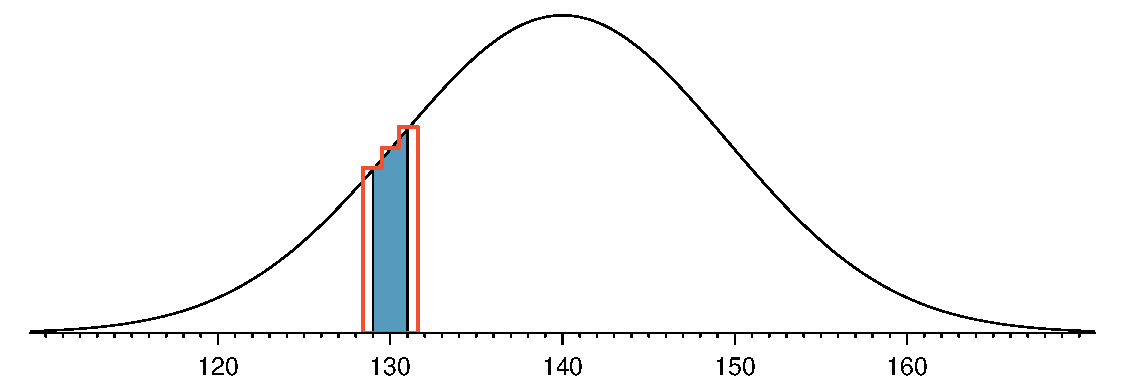
\includegraphics[width=\textwidth]{ch_distributions/figures/normApproxToBinomFail/normApproxToBinomFail-n400-p35}
\caption{A normal curve with the area between 129 and 131 shaded. The outlined area from 128.5 to 131.5 represents the exact binomial probability.}
\label{normApproxToBinomFail}
\end{figure}


\begin{onebox}{Improving accuracy of the normal approximation to the binomial distribution}
The normal approximation to the binomial distribution for intervals of values is usually improved if cutoff values for the lower end of a shaded region are reduced by 0.5 and the cutoff value for the upper end are increased by 0.5. This correction is called the continuity correction and accounts for the fact that the binomial distribution is discrete.\end{onebox}

\begin{examplewrap}
\begin{nexample}{Use the method described to find a more accurate estimate for the probability of observing 129, 130, or 131 people with blood type O+ in 400 randomly selected people when $p=0.35$.}
Instead of standardizing 129 and 131, we will standardize 128.5 and 131.5:
\begin{align*}
Z_{left} &= \frac{128.5-140}{9.5} = -1.263 \\
Z_{right} &= \frac{131.5-140}{9.5} = -0.895 \\
P(-1.263 &< Z < -0.895) = 0.0772
\end{align*}
The probability 0.0772 is much closer to the true value of 0.0732 than the previous estimate of 0.0483 we calculated using normal approximation without the continuity correction.
\end{nexample}
\end{examplewrap}

It is always possible to apply the continuity correction when finding a normal approximation to the binomial distribution. However, when $n$ is very large or when the interval is wide, the benefit of the modification is limited since the added area becomes negligible compared to the overall area being calculated.

\index{distribution!binomial!normal approximation|)}
\index{distribution!binomial|)}


\D{\newpage}

%%
\subsection*{Section summary}

\noindent In the previous chapter, we introduced the binomial formula to find the probability of exactly $x$ successes in $n$ trials for an event that has probability $p$ of success.  Instead of looking at this scenario piecewise, we can describe the entire \textit{distribution} of the number of successes and their corresponding probabilities.  
\begin{itemize}
\item The distribution of the \textit{number of successes} in $n$ independent trials gives rise to a \term{binomial distribution}.  If X has a binomial distribution with parameters $n$ and $p$, then \\
$P(X=x) = {n\choose x}p^x(1-p)^n-x$, where $x=0,1,2,3\dots,n$.

\item To write out a binomial probability \textbf{distribution table}, list all possible values for $x$, the number of successes, then use the binomial formula to find the probability of each of those values.  

\item Because a binomial distribution can be thought of as the \emph{sum} of a bunch of 0s and 1s, the \term{Central Limit Theorem} applies.  As $n$ gets larger, the shape of the binomial distribution becomes more normal.  

\item  We call the rule of thumb for when the binomial distribution can be well modeled with a normal distribution the \term{success-failure} condition.  The success-failure condition is met when there are at least 10 successes and 10 failures, or when $np\ge 10$ and $n(1-p)\ge 10$.

\item If \textit{X} follows a binomial distribution with parameters $n$ and $p$, then:
\begin{itemize}\vspace{-1mm}
\setlength{\itemsep}{0mm}
\item The mean is given by $\mu_{\scriptscriptstyle{X}} = np$. \quad (\emph{center})
\item The standard deviation is given by $\sigma_{\scriptscriptstyle{X}} = \sqrt{np(1-p)}$. \quad (\emph{spread})
\item When $np\ge 10$ and $n(1-p)\ge 10$, the binomial distribution is approximately normal.  \quad (\emph{shape})
\end{itemize}

\item It is often easier to use \termsub{normal approximation to the binomial distribution}{normal approximation!binomial distribution} rather than evaluate the binomial formula many times. These three properties of the binomial distribution are used when solving the following type of problem.  
\\
\\ \textit{Find the probability of getting more than / fewer than x yeses in $n$ trials or in a sample of size $n$}.  
\begin{enumerate}\vspace{-1mm}
\setlength{\itemsep}{0mm}
\item Identify $n$ and $p$. Verify than $np\ge 10$ and $n(1-p)\ge 10$, which implies that normal approximation is reasonable. 
\item Calculate the Z-score.  Use $\mu_{\scriptscriptstyle{X}} = np$ and $\sigma_{\scriptscriptstyle{X}} = \sqrt{np(1-p)}$ to standardize the $x$ value.  
\item Find the appropriate area under the normal curve.   
\end{enumerate}

\end{itemize}


%%%%%%%%%%Section exercises
{\exercisesheader{}

% 35

\eoce{\qt{Underage drinking, Part II\label{underage_drinking_normal_approx}} \videohref{ahss_eoce_sol-underage_drinking_normal_approx}\ \ 
We learned in Exercise~\ref{underage_drinking_intro}
that about 70\% of 18-20 year olds consumed alcoholic
beverages in any given year. We now consider a random 
sample of fifty 18-20 year olds.
\begin{parts}
\item How many people would you expect to have consumed alcoholic beverages? 
And with what standard deviation?
\item Would you be surprised if there were 45 or more people who have 
consumed alcoholic beverages?
\item What is the probability that 45 or more people in this sample have 
consumed alcoholic beverages? How does this probability relate to your answer 
to part (b)?
\end{parts}
}{}

% 36

\eoce{\qt{Chickenpox, Part II\label{chicken_pox_normal_approx}} We learned in 
Exercise~\ref{chicken_pox_intro} that about 90\% of American adults had 
chickenpox before adulthood. We now consider a random sample of 120 American 
adults.
\begin{parts}
\item How many people in this sample would you expect to have had chickenpox 
in their childhood? And with what standard deviation?
\item Would you be surprised if there were 105 people who have had chickenpox 
in their childhood?
\item What is the probability that 105 or fewer people in this sample have 
had chickenpox in their childhood? How does this probability relate to your 
answer to part (b)?
\end{parts}
}{}

% 37

\eoce{\qt{Game of dreidel\label{dreidel}} A dreidel is a four-sided spinning top 
with the Hebrew letters \textit{nun}, \textit{gimel}, \textit{hei}, and 
\textit{shin}, one on each side. Each side is equally likely to come up in a 
single spin of the dreidel. Suppose you spin a dreidel three times. Calculate 
the probability of getting

\noindent\begin{minipage}[c]{0.38\textwidth}
\begin{parts}
\item at least one \textit{nun}? 
\item exactly 2 \textit{nun}s? 
\item exactly 1 \textit{hei}? 
\item at most 2 \textit{gimel}s? \vspace{3mm}
\end{parts}
\end{minipage}%
\begin{minipage}[c]{0.32\textwidth}
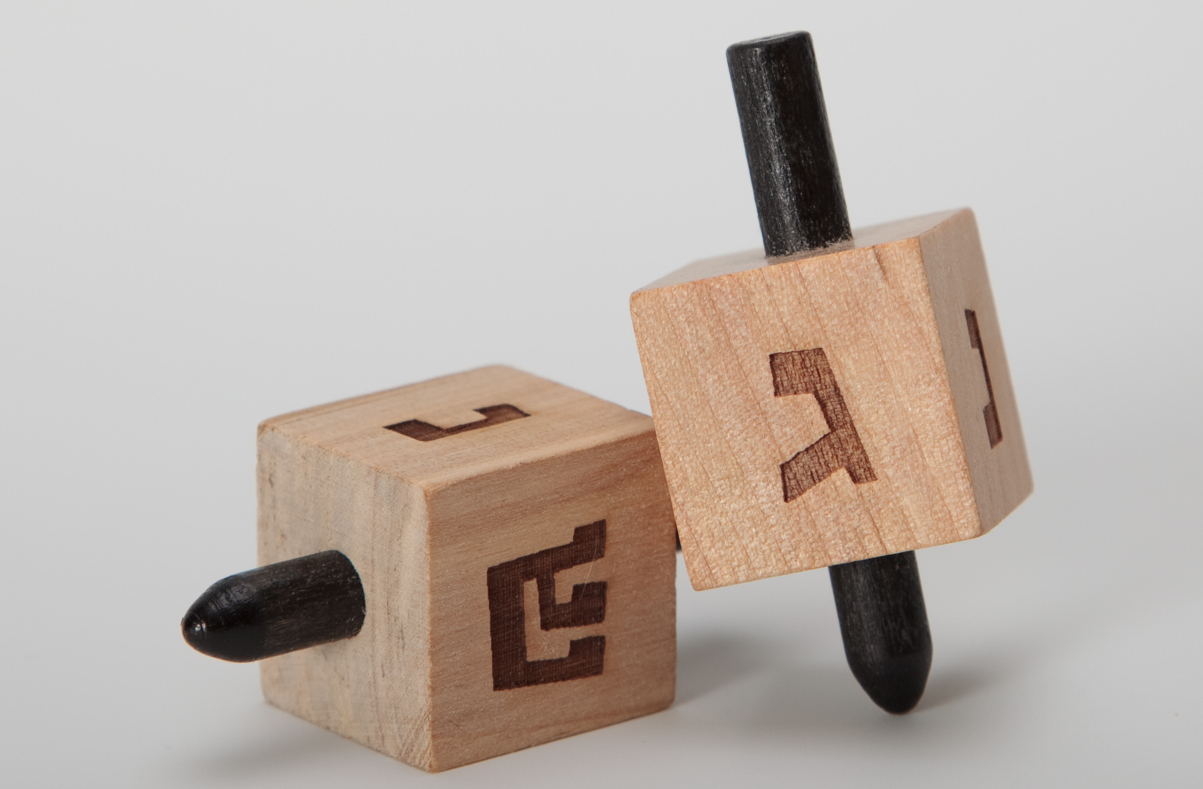
\includegraphics[width=0.9\textwidth]{ch_distributions/figures/eoce/dreidel/dreidel.jpg}
\end{minipage}%
\begin{minipage}[c]{0.28\textwidth}%
{\footnotesize Photo by Staccabees, cropped \\
  (\oiRedirect{textbook-flickr_staccabees_dreidels}{http://flic.kr/p/7gLZTf}) \\
  \oiRedirect{textbook-CC_BY_2}{CC~BY~2.0~license}} \\
\end{minipage}
}{}



% 38

\eoce{\qt{Sickle cell anemia\label{sickle_cell_anemia}} Sickle cell anemia is a 
genetic blood disorder where red blood cells lose their flexibility and 
assume an abnormal, rigid, ``sickle" shape, which results in a risk of 
various complications. If both parents are carriers of the disease, then a 
child has a 25\% chance of having the disease, 50\% chance of being a 
carrier, and 25\% chance of neither having the disease nor being a carrier. 
If two parents who are carriers of the disease have 3 children, what is the 
probability that 
\begin{parts}
\item two will have the disease?
\item none will have the disease?
\item at least one will neither have the disease nor be a carrier?
\item the first child with the disease will the be $3^{rd}$ child?
\end{parts}
}{}
}



%______________________________________________
\section[Sampling distribution of a sample proportion]{Sampling distribution of a sample proportion }
\label{distributionphat}

\sectionintro{
\noindent%
Often, instead of the number of successes in $n$ trials, we are interested in the \emph{proportion} of successes in $n$ trials.  We can use the sampling distribution of a sample proportion to answer questions such as the following:

\begin{itemize}
\item Given a population that is 50\% male, what is the probability that a random sample of 200 people would consist of less than 45\% males?

\item In a particular state, 48\% support a controversial measure.  When estimating the percent through polling, what is the probability that a random sample of size 200 will mistakenly estimate the percent support to be greater than 50\%?

\end{itemize}


%%
\subsection*{Learning objectives}
\begin{enumerate}
\setlength{\itemsep}{0mm}
\item Describe the center, spread, and shape of the sampling distribution of a sample proportion.


\item Recognize the relationship between the distribution of a sample proportion and the corresponding binomial distribution. 

\item Identify and explain the conditions for using normal approximation involving a sample proportion. Recognize that the Central Limit Theorem applies in the case of proportions/counts as well as means/sums.

\item Verify that the conditions for normal approximation are met and carry out normal approximation involving a sample proportion or sample count.

\end{enumerate}
}


%%
\subsection[The mean and standard deviation of $\hat{p}$]{The mean and standard deviation of \pmb{$\hat{p}$}}

To answer these questions, we investigate the distribution of the sample proportion $\hat{p}$. In the last section we saw that the \emph{number} of people with blood type O+ in a random sample of size 40 follows a binomial distribution with $n=40$ and $p=0.35$ that is centered on 14 and has standard deviation 3.0. What does the distribution of the \emph{proportion} of people with blood type O+ in a sample of size 40 look like?  To convert from a count to a proportion, we divide the count (i.e.~number of~yeses) by the sample size, $n = 40$. For example, 6 becomes $8/40 = 0.20$ as a proportion and 11 becomes $11/40 = 0.275$. 

We can find the general formula for the mean (expected value) and standard deviation of a sample proportion $\hat{p}$ using our tools that we've learned so far. To get the sample mean for $\hat{p}$, we divide the binomial mean $\mu_{binomial} = np$ by $n$:
\begin{align*}
\mu_{\hat{p}} = \frac{\mu_{binomial}}{n} = \frac{np}{n} = p
\end{align*}
As one might expect, the sample proportion $\hat{p}$ is centered on the true proportion $p$. Likewise, the standard deviation of $\hat{p}$ is equal to the standard deviation of the binomial distribution divided by $n$:
\begin{align*}
\sigma_{\hat{p}}
	= \frac{\sigma_{binomial}}{n}
	= \frac{\sqrt{np(1-p)}}{n}
	= \sqrt{\frac{p(1-p)}{n}}
\end{align*}

\begin{onebox}{Mean and standard deviation of a sample proportion}
The mean and standard deviation of the sample proportion describe the center and spread of the distribution of all possible sample proportions $\hat{p}$ from a random sample of size $n$ with true population proportion $p$.
\begin{align*}
\mu_{\hat{p}} &= p
	& \sigma_{\hat{p}}&= \sqrt{\frac{p(1-p)}{n}}
	\vspace{1mm}
\end{align*}\end{onebox}

%Because the distribution of $\hat{p}$ is centered at $p$, the sample proportion is said to be an \hiddenterm{unbiased estimator} of $p$.

In analyses, we think of the formula for the standard deviation of a sample proportion, $\sigma_{\hat{p}}$, as describing the uncertainty associated with the estimate $\hat{p}$. That is, $\sigma_{\hat{p}}$ can be thought of as a way to quantify the typical \hiddenterm{error} in our sample estimate $\hat{p}$ of the true proportion $p$. Understanding the variability of statistics such as $\hat{p}$ is a central component in the study of statistics.

Here, $n=40$ and $p=0.35$, $\sigma_{\hat{p}} = \sqrt{\frac{0.35(1-0.35)}{40}}=0.075$.
We see in Figure~\ref{oPositive40prop} that the distribution of number of people in a sample with blood type O+ out of 40 is equivalent to the distribution of proportion of people in a sample of size 40 with blood type O+, but with a change of scale.
Instead of counts along the horizontal axis, we have proportions.  

\begin{figure}[ht]
\centering
\subfigure[]{
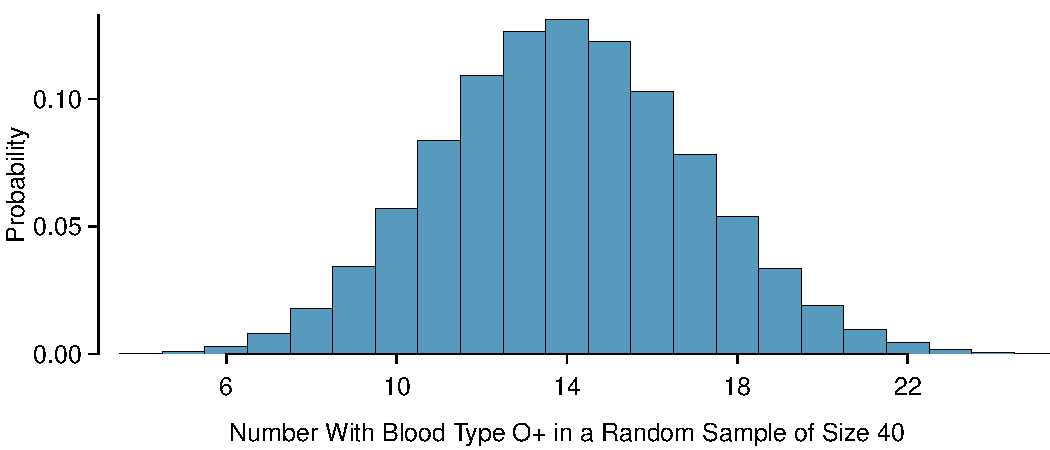
\includegraphics[width=0.475\textwidth]{ch_distributions/figures/oPositive40/oPositive40}
}
\subfigure[]{
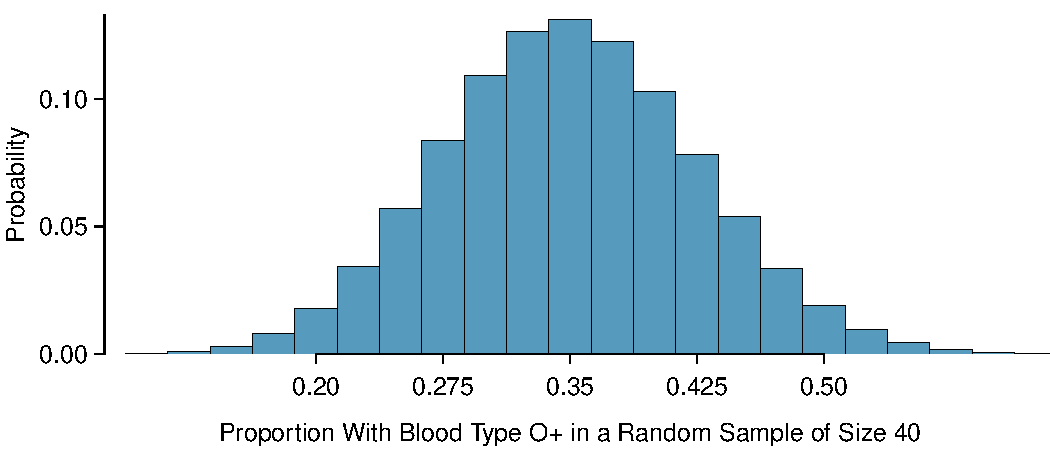
\includegraphics[width=0.475\textwidth]{ch_distributions/figures/oPositive40/oPositive40prop}
}
\caption{Two distributions where $p=0.35$ and $n=40$:  the binomial distribution for the \emph{number} with blood type O+ and the sampling distribution for the \emph{proportion} with blood type O+. }
\label{oPositive40prop}
\end{figure}


%\begin{enumerate}
%\setlength{\itemsep}{0mm}
%\item The average spread of the distribution of all possible values of $\hat{p}$ 
%\item The average \emph{error} of the sample proportion $\hat{p}$, that~is, the average deviation between a particular sample $\hat{p}$ and the true population $p$. 
%\end{enumerate}

\begin{examplewrap}
\begin{nexample}{If the proportion of people in the county with blood type O+ is really 35\%, find and interpret the mean and standard deviation of the sample proportion for a random sample of size 400.}
The mean of the sample proportion is the population proportion: 0.35. That is, if we took many, many samples and calculated $\hat{p}$, these values would average out to $p = 0.35$.

The standard deviation of $\hat{p}$ is described by the standard deviation for the proportion:
\begin{align*}
\sigma_{\hat{p}}
	= \sqrt{\frac{p(1-p)}{n}}
	= \sqrt{\frac{0.35(0.65)}{400}}
	= 0.024
\end{align*}
The sample proportion will typically be about 0.024 or 2.4\% away from the true proportion of $p = 0.35$. We'll become more rigorous about quantifying how close $\hat{p}$ will tend to be to $p$ in Chapter~\ref{foundationsForInference}.
\end{nexample}
\end{examplewrap}

%%
\subsection{The Central Limit Theorem revisited}

In section ~\ref{distributionofxbar}, we saw the Central Limit Theorem, which states that for large enough $n$, the sample mean $\bar{x}$ is normally distributed.

A natural question is, what does this have to do with sample proportions? In~fact, a~lot! A sample proportion can be written down as a sample mean. For example, suppose we have 3 successes in 10 trials. If we label each of the 3 success as a 1 and each of the 7 failures as a 0, then the sample proportion is the same as the sample mean:
\begin{align*}
\hat{p}
	= \frac{1 + 0 + 0 + 1 + 1 + 0 + 0 + 0 + 0 + 0}{10}
	= \frac{3}{10}
	= 0.3
\end{align*}
That is, the distribution of the sample proportion is governed by the Central Limit Theorem, and the Central Limit Theorem is what ties together much of the statistical theory we will see.


\begin{onebox}{Three important facts about the distribution of a sample proportion \pmb{$\hat{\MakeLowercase{p}}$}}
Consider taking a simple  random sample from a large population.
\begin{enumerate}
\setlength{\itemsep}{0mm}
\item The mean of a sample proportion is $p$.
\item The SD of a sample proportion is $\sqrt{\frac{p(1-p)}{n}}$.
\item When $np \geq 10$ and $n(1-p) \geq 10$, the sample proportion closely follows a normal distribution. 
\end{enumerate}\end{onebox}

Using these facts, we can now answer the question posed at the beginning of this section.



%%
\subsection[Normal approximation for the distribution of $\hat{p}$]{Normal approximation for the distribution of \pmb{$\hat{p}$}}

\begin{examplewrap}
\begin{nexample}{Find the probability that less than 30\% of a random sample of 400 people will be blood type O+ if the population proportion is 35\%.}
In the previous section we verified that $np$ and $n(1-p)$ are at least 10. The mean of the sample proportion is 0.35 and the standard deviation for the sample proportion is given by $\sqrt{\frac{0.35(1-0.35)}{400}}=0.024$. We can find a Z-score and use our calculator to find the probability:
\begin{align*}
Z &= \frac{\hat{p} - \mu_{\hat{p}}}{\sigma_{\hat{p}}} = \frac{0.30 - 0.35}{0.024} = -2.1 \\
P(&Z < -2.1) = 0.0179
\end{align*}
We leave it to the reader to construct a figure for this example.
\label{smokers}
\end{nexample}
\end{examplewrap}


\begin{examplewrap}
\begin{nexample}{The probability 0.0179 is the same probability we calculated when we found the probability of getting fewer than 120 with blood type O+ out of 400! Why is this?}
Notice that $120/400=0.30$. Using the binomial distribution to find the probability of fewer than 120 with blood type O+ in the sample is equivalent to using the distribution of $\hat{p}$ to find the probability of a sample proportion less than 0.30.
\end{nexample}
\end{examplewrap}


\begin{exercisewrap}
\begin{nexercise}Given a population that is 50\% male, what is the probability that a sample of size 200 would have greater than 55\% males?  Remember to verify that conditions for normal approximation are met.\footnotemark
\end{nexercise}
\end{exercisewrap}
\footnotetext{First, verify the conditions: $np = 200(0.5) = 100 \ge 10$ and $n(1-p) = 200 (0.5) = 100 \ge 10$, so the normal approximation is reasonable. Next we find the mean and standard deviation of $\hat{p}$:
\begin{align*}
\mu_{\hat{p}} &= p = 0.50
	& \sigma_{\hat{p}} &= \sqrt{\frac{p(1-p)}{n}}
		= \sqrt{\frac{0.5(0.5)}{200}}
		= 0.0354
\end{align*}
Then we find a Z-score and find the upper tail of the normal distribution:
\begin{align*}
Z = \frac{\hat{p} - \mu_{\hat{p}}}{\sigma_{\hat{p}}} = \frac{0.55 - 0.5}{0.0354} = 1.412
\qquad \rightarrow \qquad
P(Z > 1.412) = 0.07
\end{align*}
The probability of getting a sample proportion of 55\% or greater is about 0.07.}

%%
\subsection*{Section summary}

\noindent The binomial distribution shows the distribution of the number of successes in $n$ trials.  Often, we are interested in the \textit{proportion} of successes rather than the \textit{number} of successes.
\begin{itemize}
\item To convert from "number of yeses" to "proportion of yeses" we simply divide the number by $n$.  The sampling distribution of the sample proportion $\hat{p}$ is identical to the binomial distribution with a change of scale, i.e. different mean and different SD, but same shape.

\item The same \term{success-failure condition} for the binomial distribution holds for a sample proportion $\hat{p}$.

\item Three important facts about the sampling distribution of the sample proportion $\hat{p}$:
\begin{itemize}\vspace{-1mm}
\item The mean of a sample proportion is denoted by $\mu_{\hat{p}}$, and it is equal to $p$.  (\textit{center})
\item The SD of a sample proportion is denoted by $\sigma_{\hat{p}}$, and it is equal to $\sqrt{\frac{p(1-p)}{n}}$.  (\textit{spread})
\item When $np\ge 10$ and $n(1-p)\ge 10$, the distribution of the sample proportion will be approximately normal.   (\textit{shape})
\end{itemize}

\item We use these properties when solving the following type of \term{normal approximation} problem involving a sample proportion.  
\emph{Find the probability of getting more / less than $x$\% yeses in a sample of size $n$}.
\begin{enumerate}\vspace{-1mm}
\setlength{\itemsep}{0mm}
\item Identify $n$ and $p$. Verify than $np\ge 10$ and $n(1-p)\ge 10$, which implies that normal approximation is reasonable. 
\item Calculate the Z-score.  Use $\mu_{\hat{p}} = p$ and $\sigma_{\hat{p}} = \sqrt{\frac{p(1-p)}{n}}$ to standardize the sample proportion.  
\item Find the appropriate area under the normal curve.  \end{enumerate}

\end{itemize}

%%%%%%%%%%Section exercises
{\exercisesheader{}

% 39

\eoce{\qt{Distribution of $\hat{p}$} Suppose the true population proportion were $p = 0.95$. The figure below shows what the distribution of a sample proportion looks like when the sample size is $n = 20$, $n = 100$, and $n = 500$. (a) What does each point (observation) in each of the samples represent? (b) Describe the distribution of the sample proportion, $\hat{p}$. How does the distribution of the sample proportion change as $n$ becomes larger?
\begin{center}
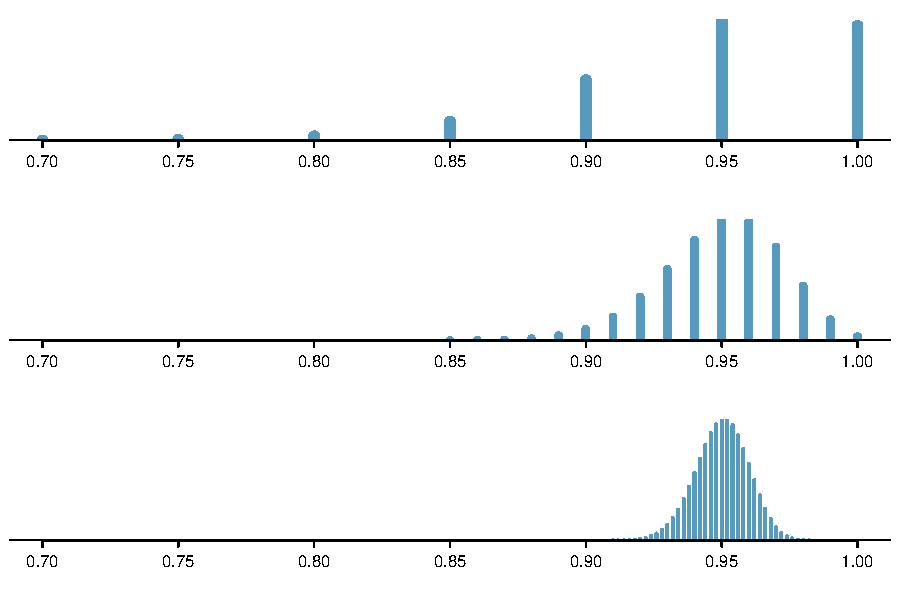
\includegraphics[width=0.85\textwidth]{ch_inference_for_props/figures/eoce/eoce-p-hat-simulations/eoce-p-hat-simulations-p95}
\end{center}}
{}

%40

\eoce{\qt{Distribution of $\hat{p}$} Suppose the true population proportion were $p = 0.5$. The figure below shows what the distribution of a sample proportion looks like when the sample size is $n = 20$, $n = 100$, and $n = 500$. What does each point (observation) in each of the samples represent? Describe how the distribution of the sample proportion, $\hat{p}$, changes as $n$ becomes larger.
\begin{center}
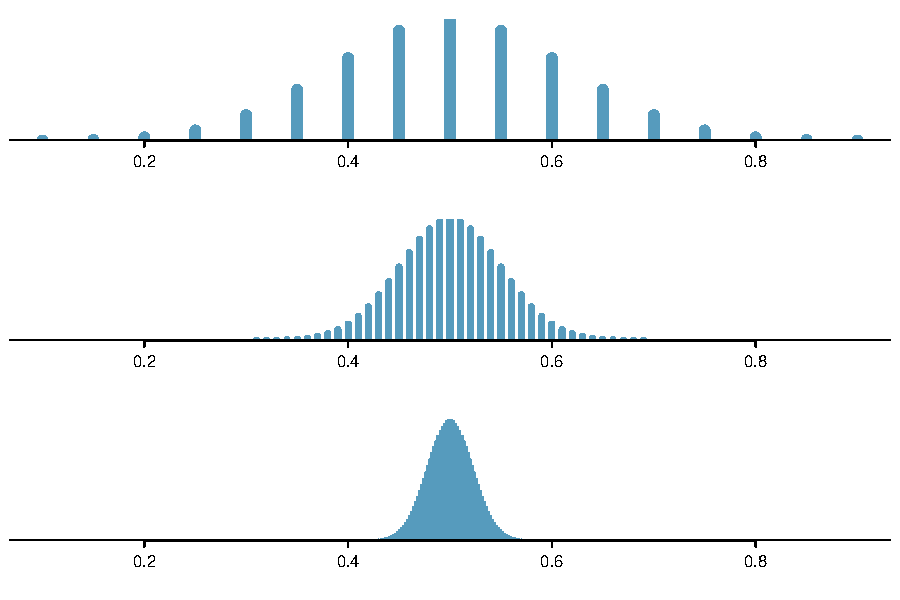
\includegraphics[width=0.85\textwidth]{ch_inference_for_props/figures/eoce/eoce-p-hat-simulations/eoce-p-hat-simulations-p5}
\end{center}}
{}

\D{\newpage}

%41

\eoce{\qt{Distribution of $\hat{p}$} \videohref{ahss_eoce_sol-distribution_of_phat}\ \ Suppose the true population proportion were $p = 0.5$ and a researcher takes a simple random sample of size $n=50$.  
\begin{parts}
\item Find and interpret the standard deviation of the sample proportion $\hat{p}$.  
\item Calculate the probability that the sample proportion will be larger than 0.55 for a random sample of size 50.
\end{parts}
}{}

%42

\eoce{\qt{Distribution of $\hat{p}$} Suppose the true population proportion were $p = 0.6$ and a researcher takes a simple random sample of size $n=50$.  
\begin{parts}
\item Find and interpret the standard deviation of the sample proportion $\hat{p}$. 
\item Calculate the probability that the sample proportion will be larger than 0.65 for a random sample of size 50.
\end{parts}
}{}

% 43

\eoce{\qt{Nearsighted children} \videohref{ahss_eoce_sol-nearsighted_children}\ \ It is believed that nearsightedness affects about 8\% of all children. We are interested in finding the probability that fewer than 12 out of 200 randomly sampled children will be nearsighted.
\begin{parts}
\item Estimate this probability using the normal approximation to the binomial distribution.
\item Estimate this probability using the distribution of the sample proportion.
\item How do your answers from parts (a) and (b) compare?
\end{parts}
}{}


% 44
\eoce{\qt{Social network use} The Pew Research Center estimates that as of January 2014, 89\% of 18-29 year olds in the United States use social networking sites.\footfullcite{data:pewsocialnetwork:2014} Calculate the probability that at least 95\% of 500 randomly sampled 18-29 year olds use social networking sites.
}{}}



%______________________________________________
\reviewchapterheader{}

\noindent This chapter began by introducing the normal distribution.  A common thread that ran through this chapter is the use of the \term{normal approximation} in various contexts.  
The key steps are included for each of the normal approximation scenarios below.

\begin{enumerate}
\item Normal approximation for \term{data}:  
\\- Verify that population is approximately normal.
\\- Use the given mean $\mu$ and SD $\sigma$ to find the Z-score for the given $x$ value.
\item Normal approximation for a \termsub{sample mean/sum}{sample mean}\index{sample sum|textbf}:  
\\Verify that population is approximately normal or that $n\ge 30$.
\\Use $\mu_{\bar{x}}=\mu$ and $\sigma_{\bar{x}}=\frac{\sigma}{\sqrt{n}}$ to find the Z-score for the given/calculated sample mean.
\item Normal approximation for the \term{number of successes} (binomial):  
\\- Verify that $np\ge 10$ and $n(1-p)\ge 10$.
\\- Use $\mu_{\scriptscriptstyle{X}} = np$ and $\sigma_{\scriptscriptstyle{X}} = \sqrt{np(1-p)}$ to find the Z-score for the given number of successes.  
\item Normal approximation for a \term{sample proportion}:  
\\- Verify that $np\ge 10$ and $n(1-p)\ge 10$.
\\- Use $\mu_{\hat{p}} = p$ and $\sigma_{\hat{p}} = \sqrt{\frac{p(1-p)}{n}}$ to find the Z-score for the given sample proportion.
\item Normal approximation for the \term{sum of two independent random variables}:
\\- Verify that each random variable is approximately normal.
\\- Use $E(X+Y)=E(X)+E(Y)$ and $SD(X+Y)=\sqrt{(SD(X))^2+(SD(Y))^2}$ to find the Z-score for the given sum.
\end{enumerate}
Cases 1 and 2 apply to \term{numerical} variables, while cases 3 and 4 are for \term{categorical} yes/no variables.  Case 5 applies to both numerical and categorical variables.
\\
\\Note that in the binomial case and in the case of proportions, we never look to see if the \emph{population} is normal.  That would not make sense because the ``population" is simply a bunch of no/yes, 0/1 values and could not possibly be normal.
\\
\\The \term{Central Limit Theorem} is the mathematical rule that ensures that when the sample size is sufficiently large, the sample mean/sum and sample proportion/count will be approximately normal.  

